\documentclass{article}
\usepackage[english]{babel}
\usepackage[a4paper, total={6in, 8in}]{geometry}
\usepackage{fancyhdr}
\setlength{\parskip}{0.5em} % Leave space after each paragraph
\setlength{\parindent}{0ex} % Set paragraph indent to 0

% Citation
\usepackage[numbers]{natbib}

% Mathematics packages
\usepackage{amsthm, amsmath, amssymb, amsfonts, nicefrac, mathpazo} 
\newtheorem{mydef}{Definition}
\usepackage{diagbox} %Diagonal boxes in tables

% Images
\usepackage{graphicx}
\graphicspath{ {../images/} }
\usepackage{subcaption}
\usepackage{csquotes}
%\numberwithin{equation}{section} % Number equations with decimals of section they are under

% Coding colours
\usepackage{color}
\definecolor{codegreen}{rgb}{0,0.6,0}
\definecolor{codegray}{rgb}{0.5,0.5,0.5}
\definecolor{codepurple}{rgb}{0.58,0,0.82}
\definecolor{backcolour}{rgb}{0.95,0.95,0.92}
\definecolor{codeblue}{rgb}{0,0,1}
 
% Coding style
\usepackage{listings}
\lstdefinestyle{mystyle}{
    backgroundcolor=\color{backcolour},   
    commentstyle=\color{codegreen},
    keywordstyle=\color{codeblue},
    numberstyle=\tiny\color{codegray},
    stringstyle=\color{codepurple},
    basicstyle=\footnotesize,
    breakatwhitespace=false,         
    breaklines=true,                 
    captionpos=b,                    
    keepspaces=true,                 
    numbers=left,                    
    numbersep=5pt,                  
    showspaces=false,                
    showstringspaces=false,
    showtabs=false,                  
    tabsize=2
}
\lstset{style=mystyle}

% Easier to call Naturals, Integers and so on.
\newcommand{\N}{\mathbb{N}}
\newcommand{\Z}{\mathbb{Z}}
\newcommand{\Q}{\mathbb{Q}}
\newcommand{\C}{\mathbb{C}}
\newcommand{\ind}{1\hspace{-2.1mm}{1}} %Indicator Function
\newcommand{\I}{\mathtt{i}}
\newcommand{\EE}{\mathbb{E}}
\newcommand{\RR}{\mathbb{R}}
\newcommand{\PP}{\mathbb{P}}
\newcommand{\D}{\mathrm{d}}
\newcommand{\Xe}{X^{\varepsilon}}
\newcommand{\E}{\mathrm{e}}
\newcommand{\Tr}{\mathrm{Tr}}
\newcommand{\HH}{\mathrm{H}}
\newcommand{\sgn}{\mathrm{sgn}}
\newcommand{\atanh}{\mathrm{arctanh}}
\newcommand{\Lagr}{\mathcal{L}}
\def\equalDistrib{\,{\buildrel \Delta \over =}\,}
\DeclareMathOperator*{\argmin}{argmin}
\DeclareMathOperator*{\argmax}{argmax} 

% Writing Algorithms
\usepackage[]{algpseudocode}

%%%%%%%%%%%%%%%%%%%%%%%%%%%%%%%%%%%%%%%%%%%%%%%%%%%%%%%%%%%%
\cfoot{\thepage}

%%%%%%%%%%%%%%%%%%%%%%%%%%%%%%%%%%%%%%%%%%%%%%%%%%%%%%%%%%%%
\begin{document}

%%%%%%%%%%%%%%%%%%%%%%%%%%%%%%%%%%%%%%%%%%%%%%%%%%%%%%%%%%%%
\begin{center}
    
    {\Huge Computation PDEs: Project 3}\\
    {\Huge An Annular Model of Planetary Convection}
    \vspace{0.5cm}
    
    {\LARGE Yadu \emph{Bhageria}}\\
    \vspace{0.2cm}
    
\end{center}

%%%%%%%%%%%%%%%%%%%%%%%%%%%%%%%%%%%%%%%%%%%%%%%%%%%%%%%%%%%%
In this final project the Convection Equations for annular flow are considered in terms of polar coordinates $(r, \theta)$. This is a simplified model of thermally driven convection between two spheres.

\begin{align}
	T_t + \textbf{u} \cdot \nabla T &= \nabla^2 T \\
	P_r^{−1} (\textbf{u} + \textbf{u} \cdot \nabla \textbf{u}) &= − \nabla p − R_a T\hat{g} + \nabla^2 \textbf{u} \\
	\nabla \textbf{u} &= 0
\end{align}

The domain is restricted to $1 < r < b$ and is split into a grid of size $(M+1) \times N$. Therefore $\delta r = \frac{b-1}{M}$ and $\delta \theta = \frac{2 \pi}{N}$. Results in Project 2 suggested that a more efficient way to get accurate results is to have $\frac{M}{N} < 1$ rather than have $M=N$. Thus I have maintained $\frac{M}{N} = \frac{1}{4}$ throughout Project 3 as well unless testing for the impact of varying $M$ or $N$ on the error. 

The temperature boundary conditions are $T = 1$ on $r = 1$ and $T = 0$ on $r = b$. The boundaries $r=1$ and $r=b$ are mentioned together as $\partial \Omega$ in the rest of the report. 

\texttt{plotAnnulusScalarField.m} and \texttt{plotAnnulusVectorField.m} have been used throughout the project to plot the graphs.

The figures are at the end of the written assignment rather than incorporated through it for easier flow of reading. They have been referenced by Figure name where applicable.

%%%%%%%%%%%%%%%%%%%%%%%%%%%%%%%%%%%%%%%%%%%%%%%%%%%%%%%%%%%%
\section{Advection}

First we try to advect a quantity $Q(r,\theta, t)$ by $Q_t + \textbf{u} \cdot \nabla Q = 0$ such that it is second order in space and time. In polar co-ordinates we have that

\begin{equation}
	\nabla Q = \frac{\partial Q}{\partial r} \boldsymbol{\hat{r}} + \frac{1}{r} \frac{\partial Q}{\partial \theta} \boldsymbol{\hat{\theta}}
\end{equation}

$Q(r, \theta)$ is a scalar field and $\nabla$ is the del operator. Joining this with a velocity vector field \textbf{u}$(r, \theta) = u_{(r)} \boldsymbol{\hat{r}} + u_{(\theta)} \boldsymbol{\hat{\theta}}$ we get that

\begin{equation}
	\textbf{u} \cdot \nabla Q = u_{(r)} \frac{\partial Q}{\partial r} + u_{(\theta)} \frac{1}{r} \frac{\partial Q}{\partial \theta}
\end{equation}

Now $Q$ can be advected by solving the given equation $Q_t = - \textbf{u} \cdot \nabla Q$ using Richtmyer's second-order Lax-Wendroff routine. This is done in \texttt{annulusAdvect.m}. This function assumes that $Q = \Omega_1(\theta)$ and $Q = \Omega_b(\theta)$ as well as that $\textbf{u} = 0$ on the boundaries, $\partial \Omega$.

A suitable velocity field is found by deriving it from a stream function, $\psi$, using the relations 

\begin{align*}
	u_{(r)} &= \frac{\psi_\theta}{r} \\
	u_{(\theta)} &= \psi_r
\end{align*}

I have chosen a non uniform stream function (Equation \ref{eq:psi1}) that obeys $\psi = \psi_r = 0$ on the boundaries $\partial \Omega$. This can be visualized in the Figure \ref{fig:q1psi}.

\begin{align}
	\psi(r, \theta) = e^{- \left(r - \frac{b}{2}\right)^2} e^{ - (\theta - \pi)^2 } (r-1)^2 (r-b)^2
	\label{eq:psi1}
\end{align}

The initial non uniform temperature chosen is as in Equation \ref{eq:T1}. This is shown in first image of Figure \ref{fig:q1Advect} or the first image of Figure \ref{fig:q1Compare}.

\begin{align}
	Q_0(r, \theta) = .01 \sin(\pi r) \sin(\theta)
	\label{eq:T1}
\end{align}

	%%%%%%%%%%%%%%%%%%%%%%%%%%%%%%%%%%%%%%%%%%%%%%%%%%%%%%%%%%%%
	\begin{figure}[h!]
		\centering
		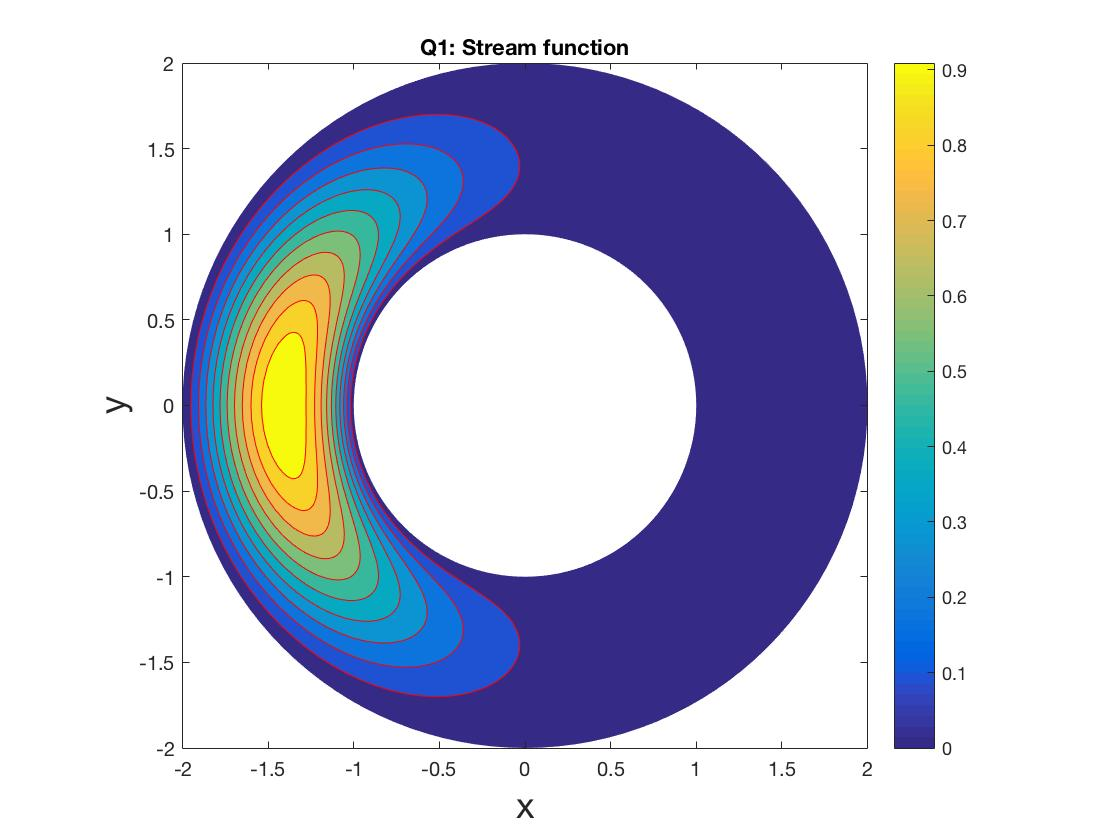
\includegraphics[width = \textwidth]{fig_q1_psi}
		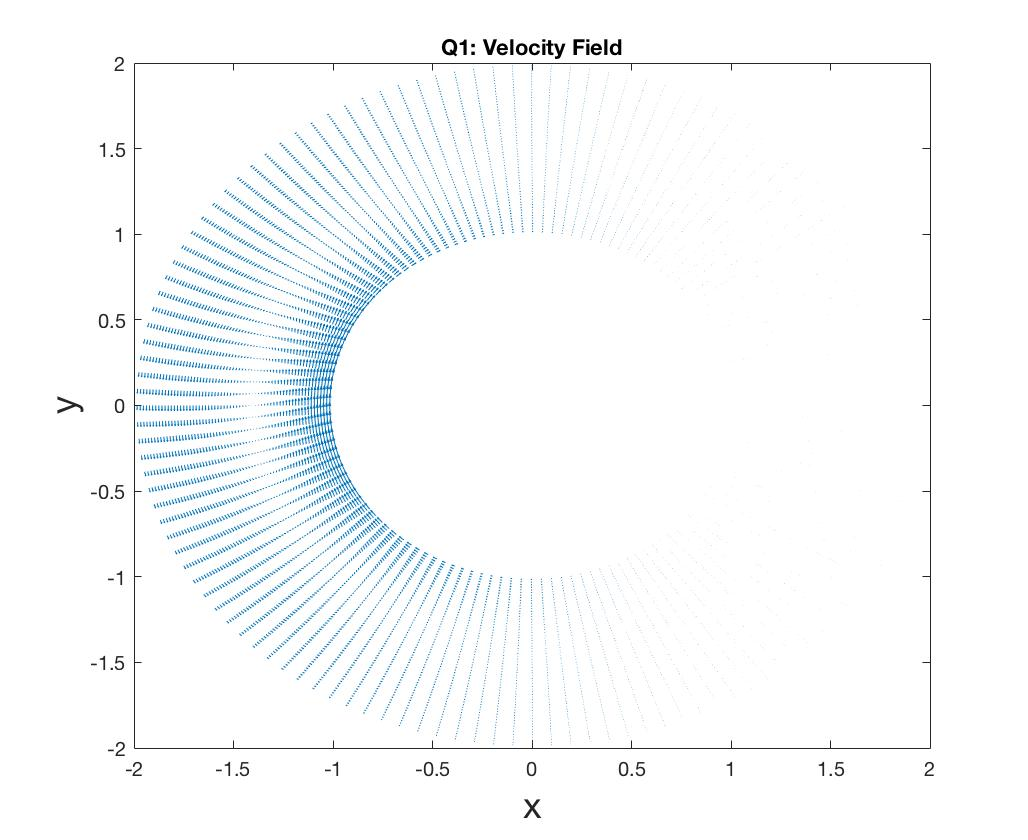
\includegraphics[width = \textwidth]{fig_q1_u}
		\caption{The stream function, $\psi$, and the corresponding velocity field, $\textbf{u}$, chosen for Q1 with $b=2$}
		\label{fig:q1psi}
	\end{figure}
	%%%%%%%%%%%%%%%%%%%%%%%%%%%%%%%%%%%%%%%%%%%%%%%%%%%%%%%%%%%%
%	%%%%%%%%%%%%%%%%%%%%%%%%%%%%%%%%%%%%%%%%%%%%%%%%%%%%%%%%%%%%
%	\begin{figure}[h!]
%		\centering
%		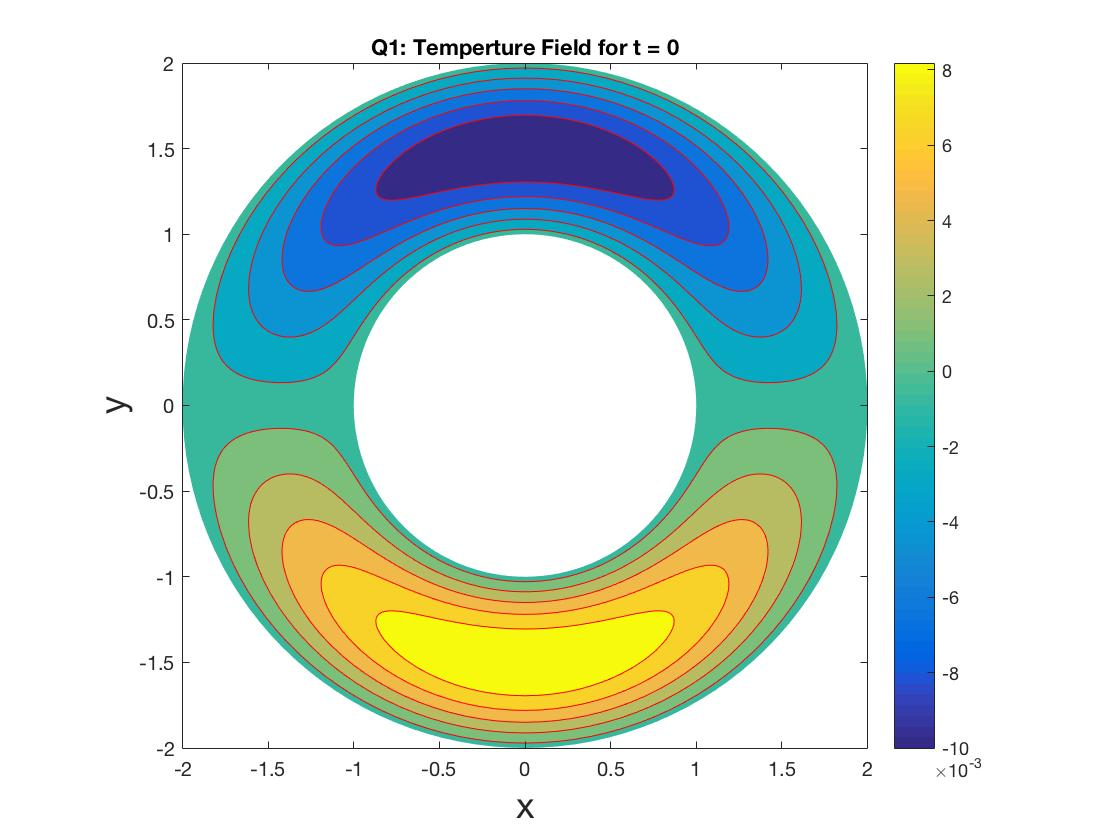
\includegraphics[width = 0.8\textwidth]{fig_q1_Q0}
%		\caption{The Temperature Field, $Q_0$, at time zero chosen for Q1 with $b=2$}
%		\label{fig:q1Q0}
%	\end{figure}
%	%%%%%%%%%%%%%%%%%%%%%%%%%%%%%%%%%%%%%%%%%%%%%%%%%%%%%%%%%%%%

Advecting this field forward in time is shown in Figure \ref{fig:q1Advect}. I chose values of $M = 2^6$, $N=2^8$, $\delta t = 0.01 \min(\delta r, \delta \theta)$ and number of time steps $= 10000$. It can be seen, by considering the velocity field given in Figure \ref{fig:q1psi}, that the quantity $Q$ follows the vectors of the velocity field, \textbf{u}. Furthermore, advecting the quantity $Q$ back in time returns it to its initial state that is visually indistinguishable (Figure \ref{fig:q1Compare}) but has some small error. The errors in this specific case are

\begin{verbatim}
max_error =
   1.6651e-06

average_error =
   1.0875e-09
\end{verbatim}

where max error $= \max_{r,\theta}(|Q_0 - \hat{Q}|)$ and average error $= \frac{|Q_0 - \hat{Q}|}{(M-1)N}$. Note that $Q(1,:)$ and $Q(M+1,:)$ are not changed by the advection function.

	%%%%%%%%%%%%%%%%%%%%%%%%%%%%%%%%%%%%%%%%%%%%%%%%%%%%%%%%%%%%
	\begin{figure}[h!]
		\centering
		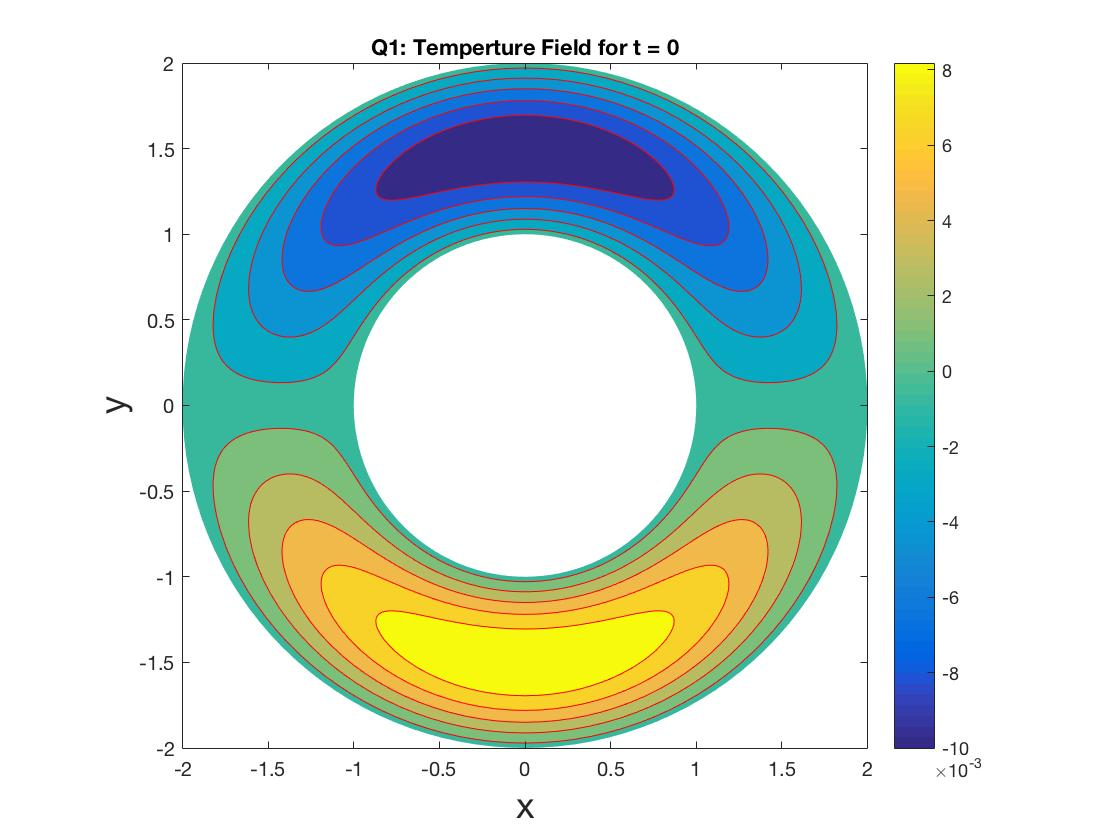
\includegraphics[width = 0.49\textwidth]{fig_q1_Q0}
		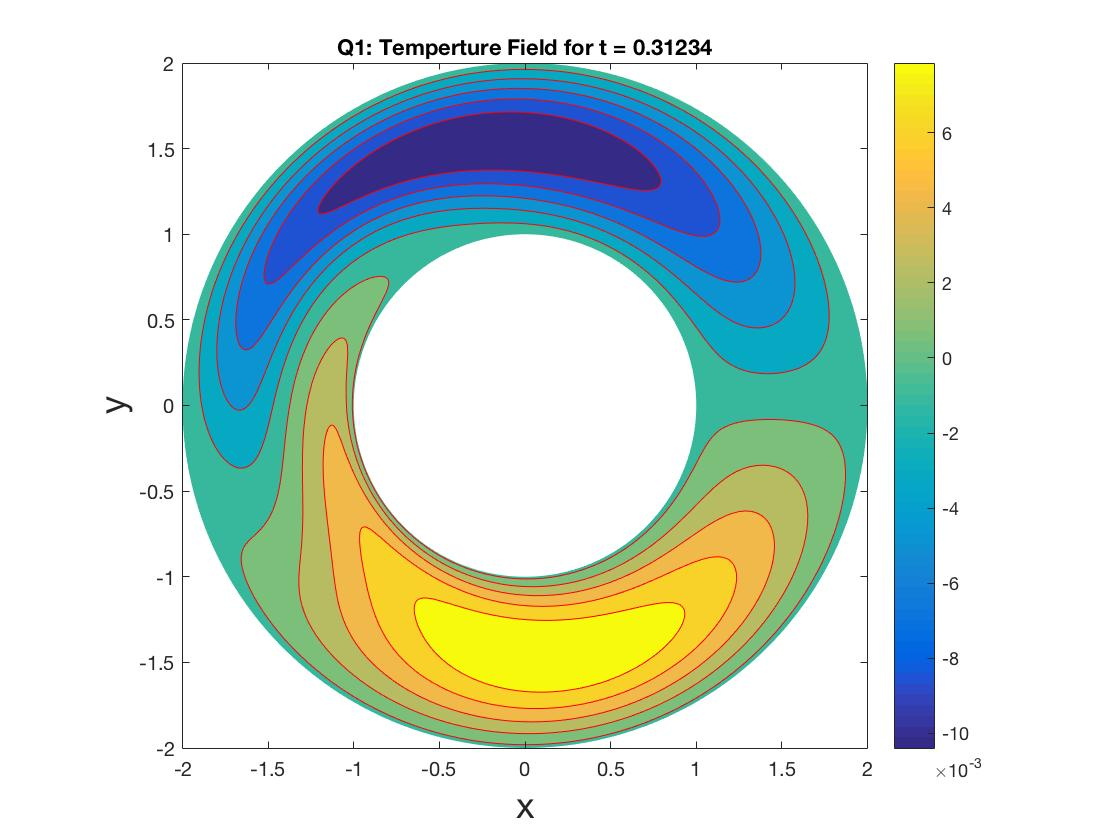
\includegraphics[width = 0.49\textwidth]{fig_q1Advect2}
		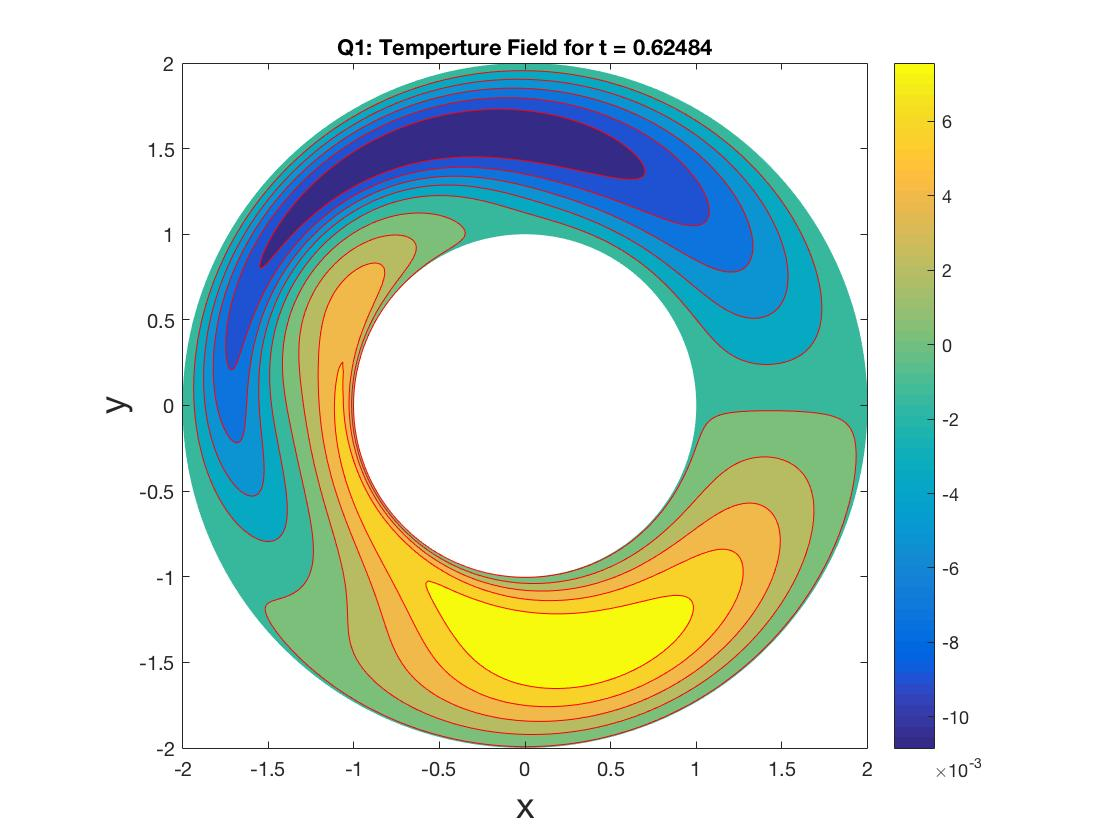
\includegraphics[width = 0.49\textwidth]{fig_q1Advect4}
		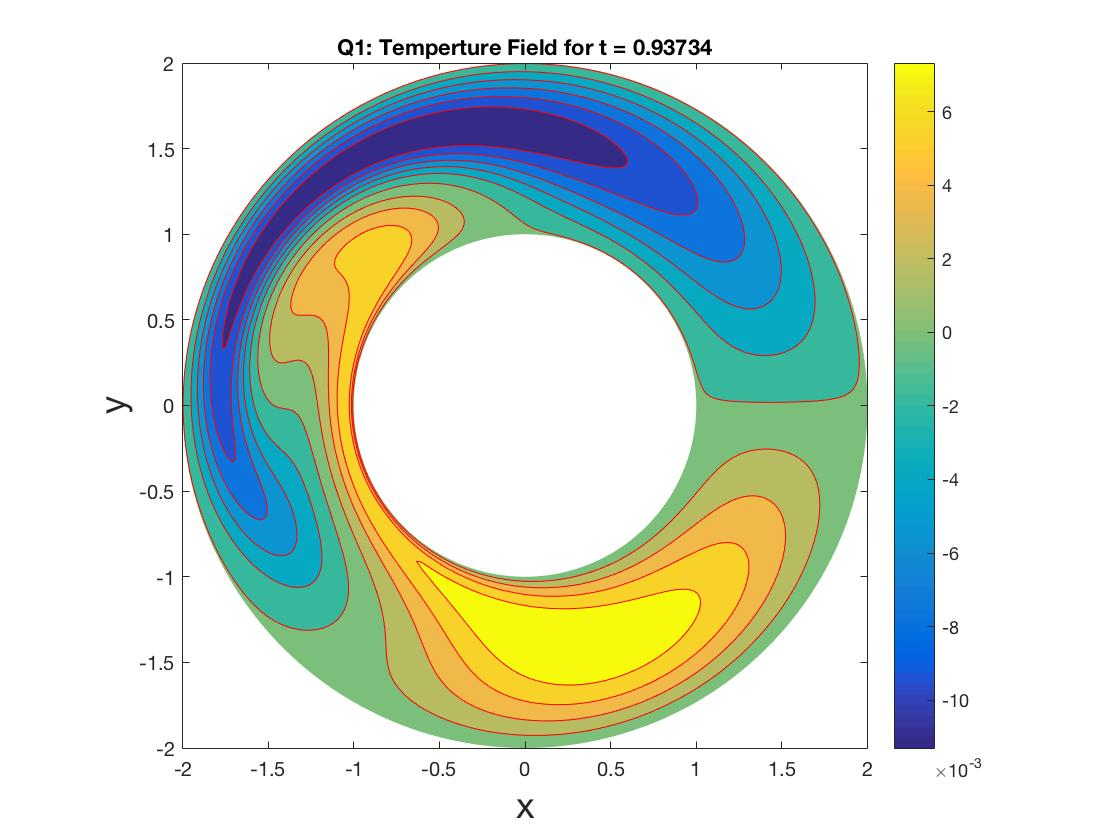
\includegraphics[width = 0.49\textwidth]{fig_q1Advect6}
		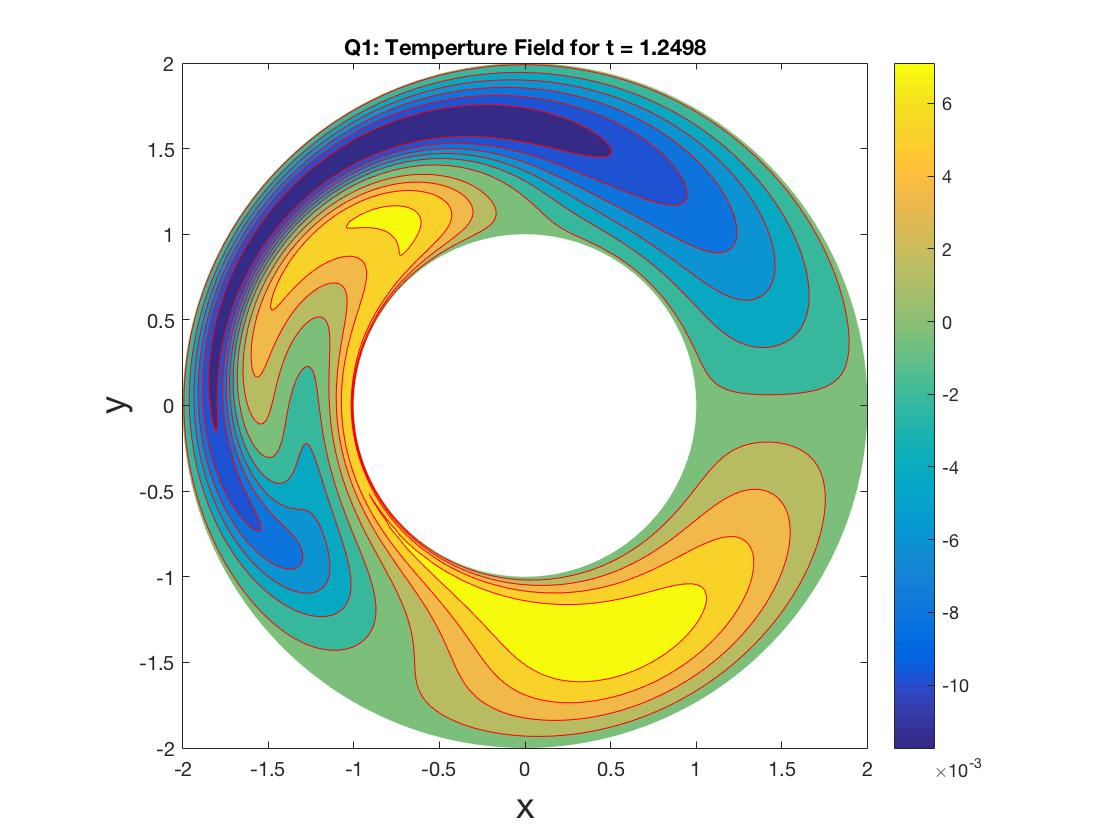
\includegraphics[width = 0.49\textwidth]{fig_q1Advect8}
		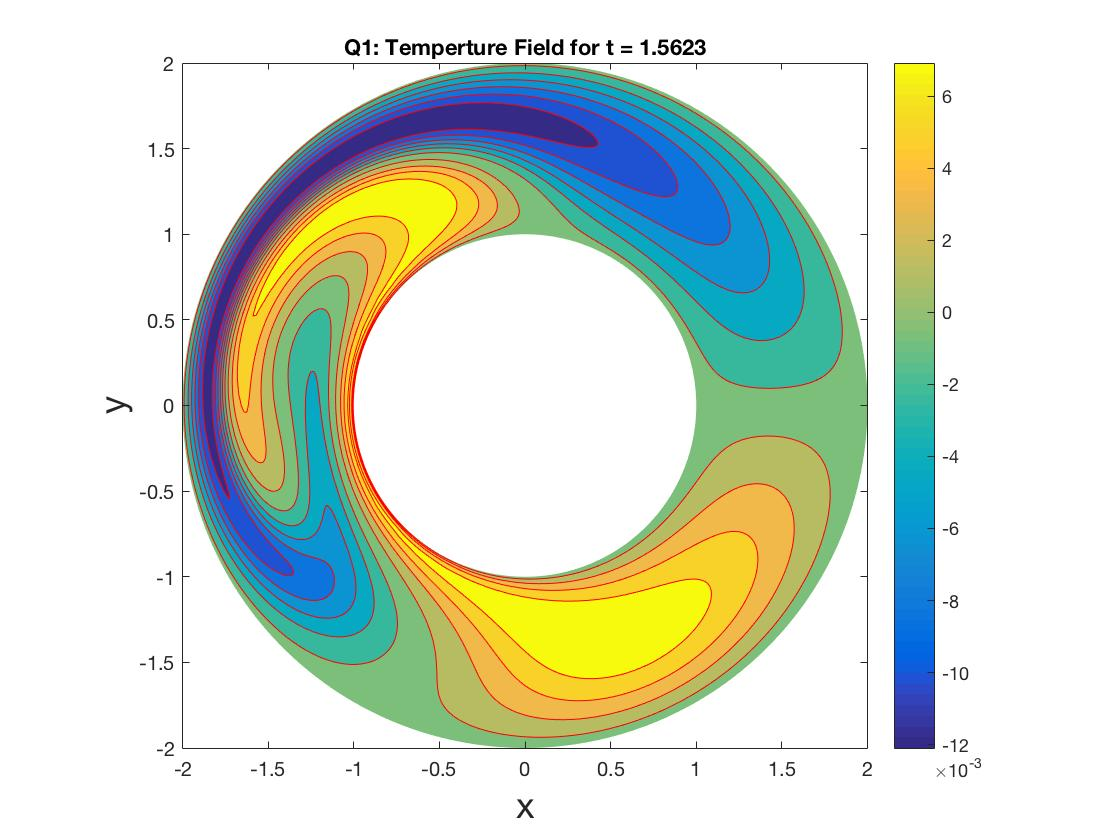
\includegraphics[width = 0.49\textwidth]{fig_q1Advect10Final}
		\caption{Advecting the specified field $Q_0$ for $\delta t = 1.5625e-04$ and tstep $= 10000$ with $M = 2^6$ and $N=2^8$}
		\label{fig:q1Advect}
	\end{figure}
	%%%%%%%%%%%%%%%%%%%%%%%%%%%%%%%%%%%%%%%%%%%%%%%%%%%%%%%%%%%%
	
		%%%%%%%%%%%%%%%%%%%%%%%%%%%%%%%%%%%%%%%%%%%%%%%%%%%%%%%%%%%%
	\begin{figure}[h!]
		\centering
		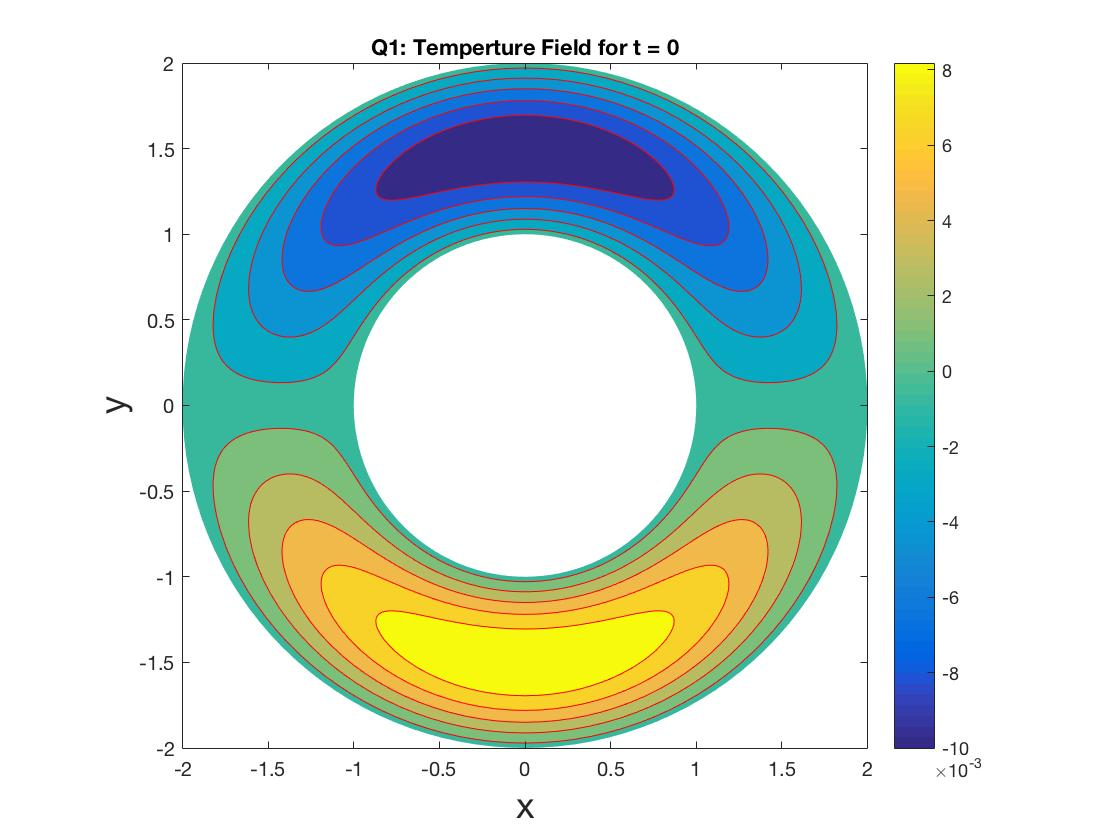
\includegraphics[width = 0.49\textwidth]{fig_q1_Q0}
		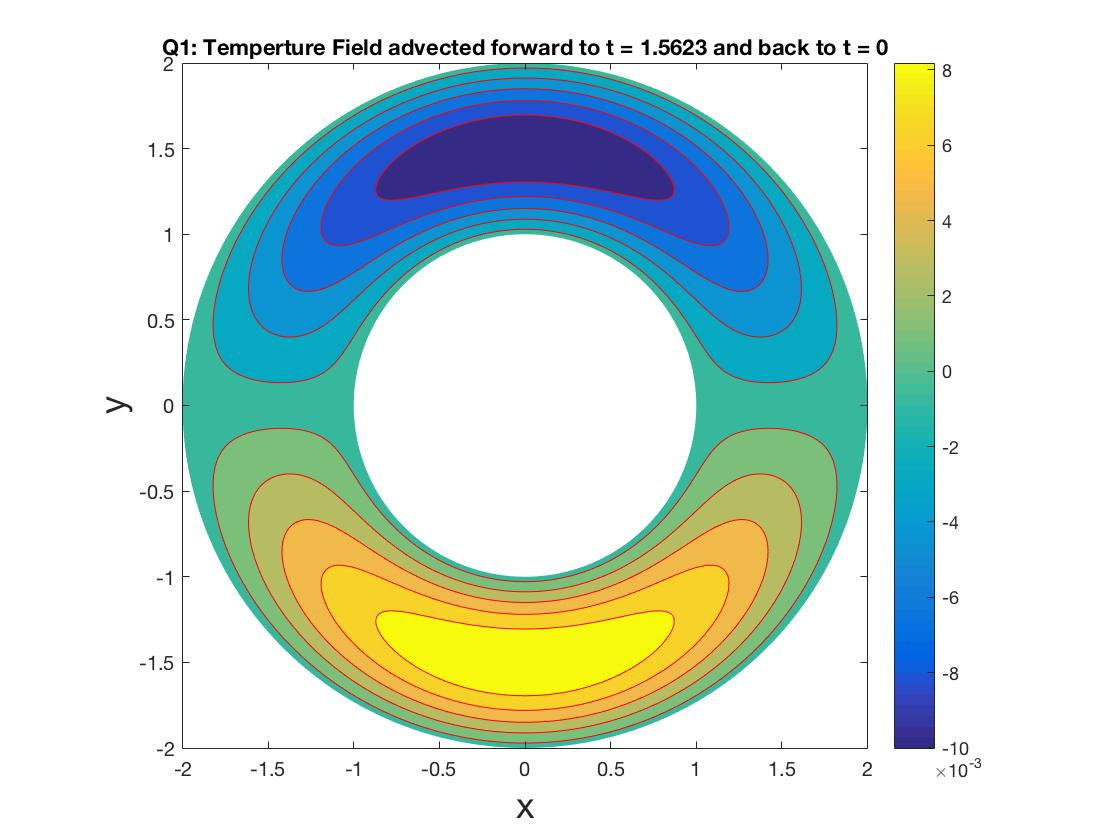
\includegraphics[width = 0.49\textwidth]{fig_q1AdvectBack}
		\caption{Comparison of the initial quantity $Q_0$ and the quantity advected forwards to $t = \delta t \cdot $ tstep and then back again to $t=0$. Parameters are $\delta t = 1.5625e-04$ and tstep $= 10000$ with $M = 2^6$ and $N=2^8$.}
		\label{fig:q1Compare}
	\end{figure}
	%%%%%%%%%%%%%%%%%%%%%%%%%%%%%%%%%%%%%%%%%%%%%%%%%%%%%%%%%%%%

 Thus the routine seems to be functioning as intended. These results can be reproduced using \texttt{q1.m}.
 
	%%%%%%%%%%%%%%%%%%%%%%%%%%%%%%%%%%%%%%%%%%%%%%%%%%%%%%%%%%%%
	\begin{figure}[h!]
		\centering
		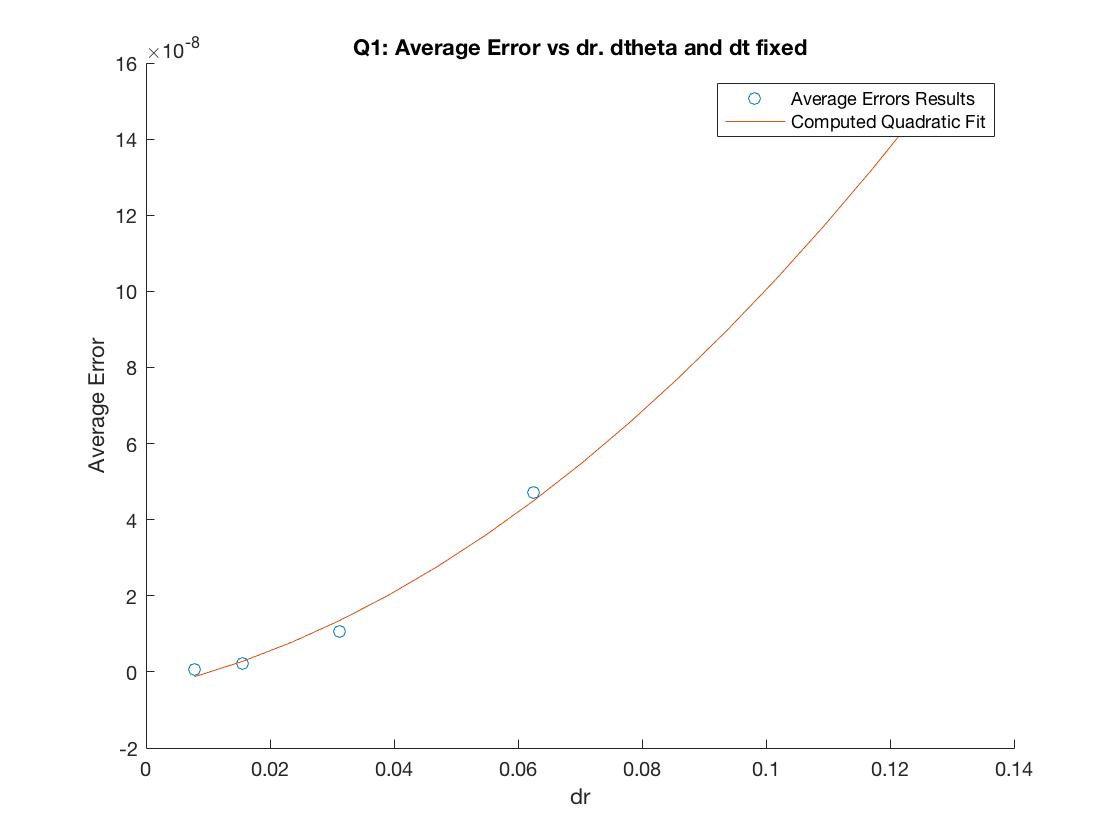
\includegraphics[width = 0.49\textwidth]{fig_q1_dr}
		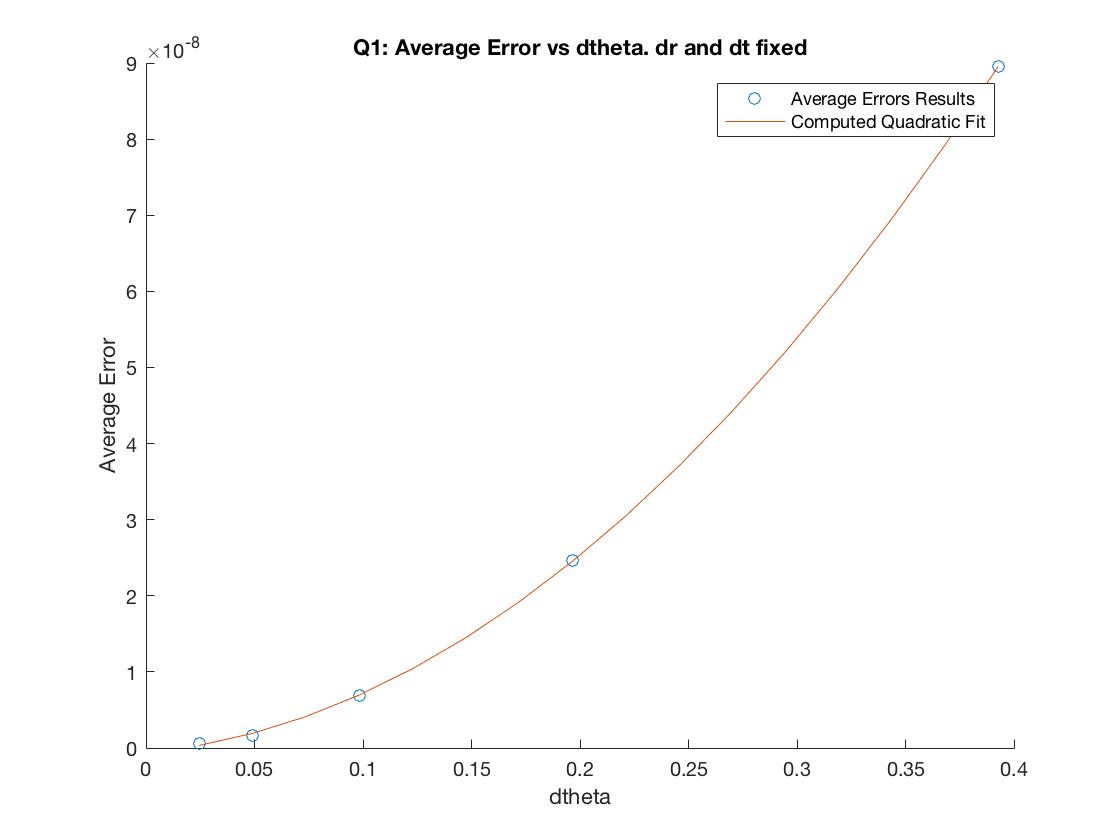
\includegraphics[width = 0.49\textwidth]{fig_q1_dtheta}
		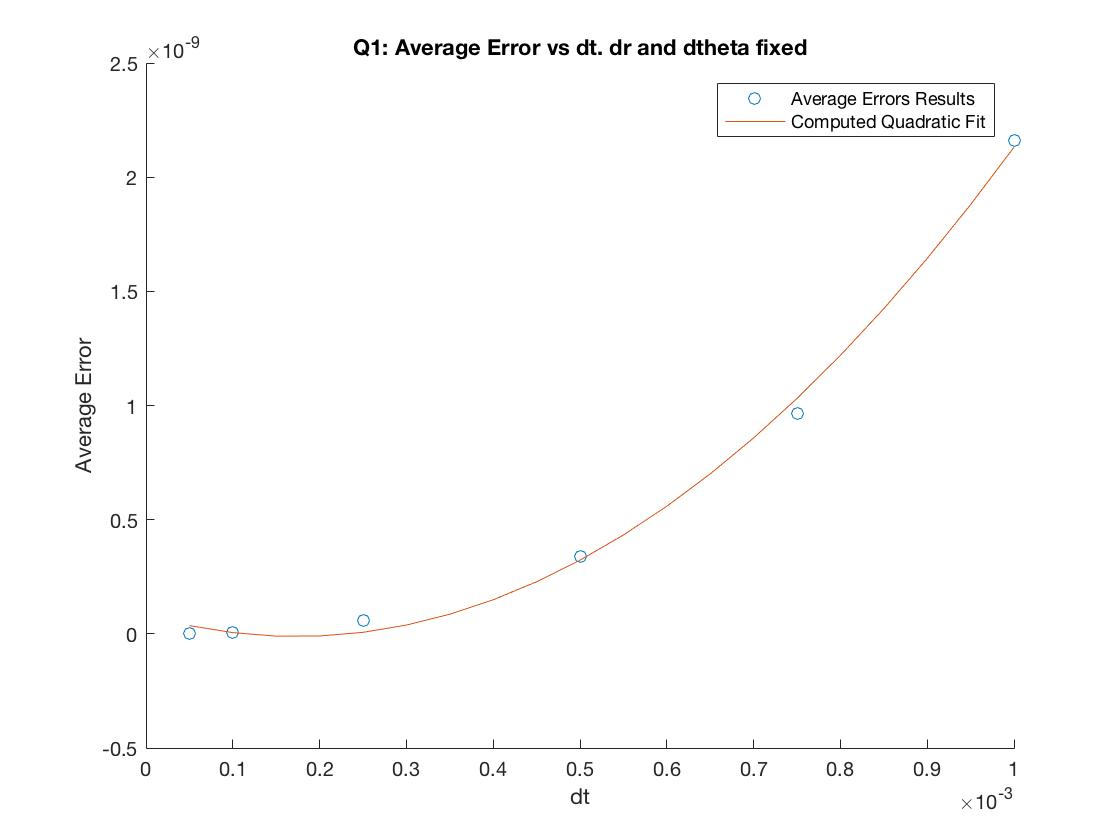
\includegraphics[width = 0.49\textwidth]{fig_q1_dt}
		\caption{Average Error plots for varying $\delta r, \delta \theta, \delta t$ one at a time.}
		\label{fig:q1Errors}
	\end{figure}
	%%%%%%%%%%%%%%%%%%%%%%%%%%%%%%%%%%%%%%%%%%%%%%%%%%%%%%%%%%%%

\subsection{Check that the Routine is 2nd Order in Space and Time}

Now we need to check whether this routine is 2nd order in space and time. That is the errors should be $\mathcal{O}(\delta r^2,\delta \theta^2,\delta t^2)$. This can be done by keeping two of the three values out of $\delta r, \delta \theta, \delta t$ constant and varying the other to find various values for the average error. Then the inbuilt MATLAB function can be used to fit this data to a polynomial of order 2 to make sure that the average error results are indeed 2nd order. I have implemented this in \texttt{q1ErrorPlots.m} that also calls \texttt{q1Errors.m}. The results can be seen in Figure \ref{fig:q1Errors} that demonstrate the 2nd order behaviour of the implemented routine.

%%%%%%%%%%%%%%%%%%%%%%%%%%%%%%%%%%%%%%%%%%%%%%%%%%%%%%%%%%%%
\newpage
\section{Diffusion}

Now we wish to diffuse a quantity by $Q_t = \nabla^2 Q$. This can be done using the MultiGrid routine formulated in project 2 with revised Dirichlet boundary conditions and revised Gauss-Seidel and residual update steps. Using the Crank-Nicolson routine, we can write

\begin{align}
	Q^{(i+1)} - \frac{\delta t}{2} \nabla^2 Q^{(i+1)} &= Q^{(i)} + \frac{\delta t}{2} \nabla^2 Q \\
\end{align}

This can be written in the simplified form

\begin{align*}
	Q^{(i+1)} - \frac{\delta t}{2} \nabla^2 Q^{(i+1)} &= f
\end{align*}

where $f$ is easily computable (done in \texttt{T\_delsqr.m}). \texttt{T\_MultiGrid.m}, \texttt{T\_GaussSeidel.m}, and \texttt{T\_residual.m} are used to then compute $Q^{(i+1)}$ by solving the system $A Q^{(i+1)} = f$ where $A = I - \frac{\delta t}{2} \nabla^2$. 

To make sure the routine is working properly, we use a similar quantity $Q_0$ defined above (in Equation \ref{eq:T1}) but multiplied by $100$ and with added boundary condition of $Q_0(1,:) = 1$. We then advect this quantity using the function \texttt{annulusAdvect.m} until the maximum error between each iteration drops below a specified tolerance. This is done in \texttt{q2DiffuseTest.m} with the same values of $M=2^6, N=2^8,$ and $\delta t = 0.01 \min(\delta r, \delta \theta) $ as in \texttt{q1.m} along with a tolerance level of $10^{-5}$. The results can be seen in Figure \ref{fig:q2DiffuseTest} which agree with the expected intuition of the annulus tending to a linear gradient from $r=1$ to $r=b$ normalizing any initial perturbations due to the Dirichlet boundary conditions of $Q_0(1,:) = 1$ and $Q_0(b,:) = 0$. That is the quantity moves from areas of high concentration to areas of low concentration.

	%%%%%%%%%%%%%%%%%%%%%%%%%%%%%%%%%%%%%%%%%%%%%%%%%%%%%%%%%%%%
	\begin{figure}[h!]
		\centering
		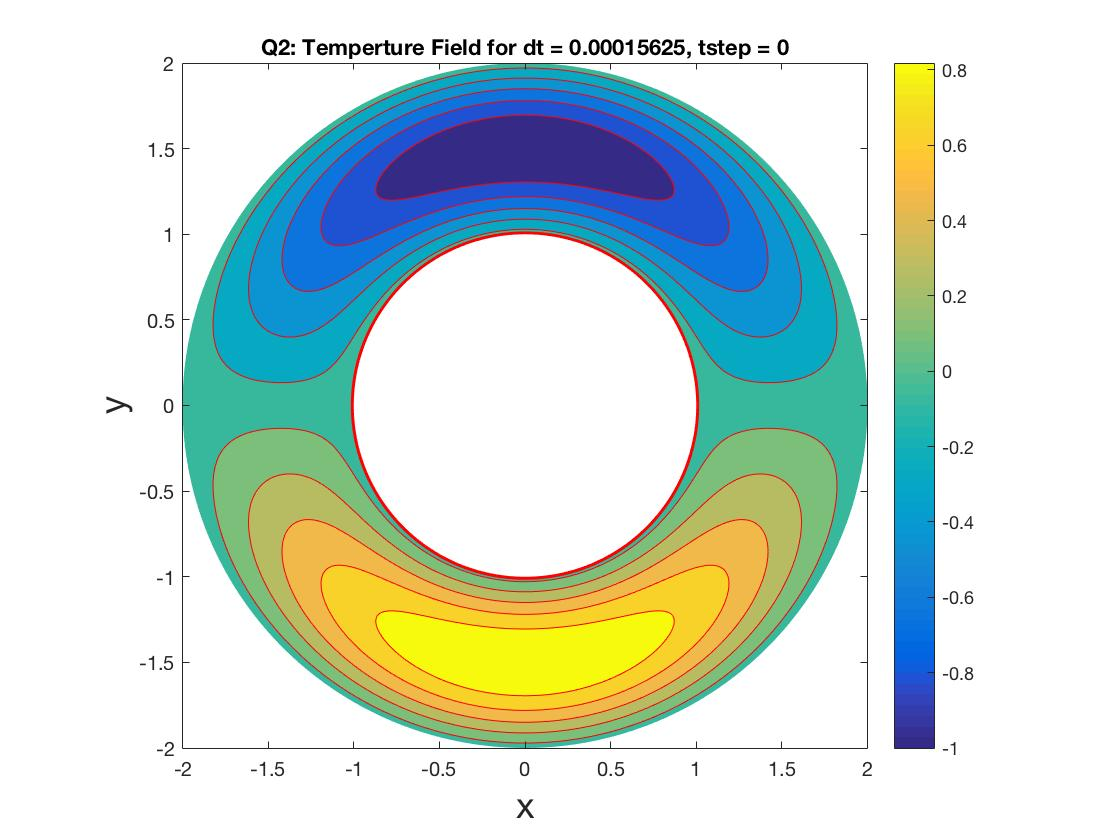
\includegraphics[width = 0.49\textwidth]{fig_q2DiffuseTest0}
		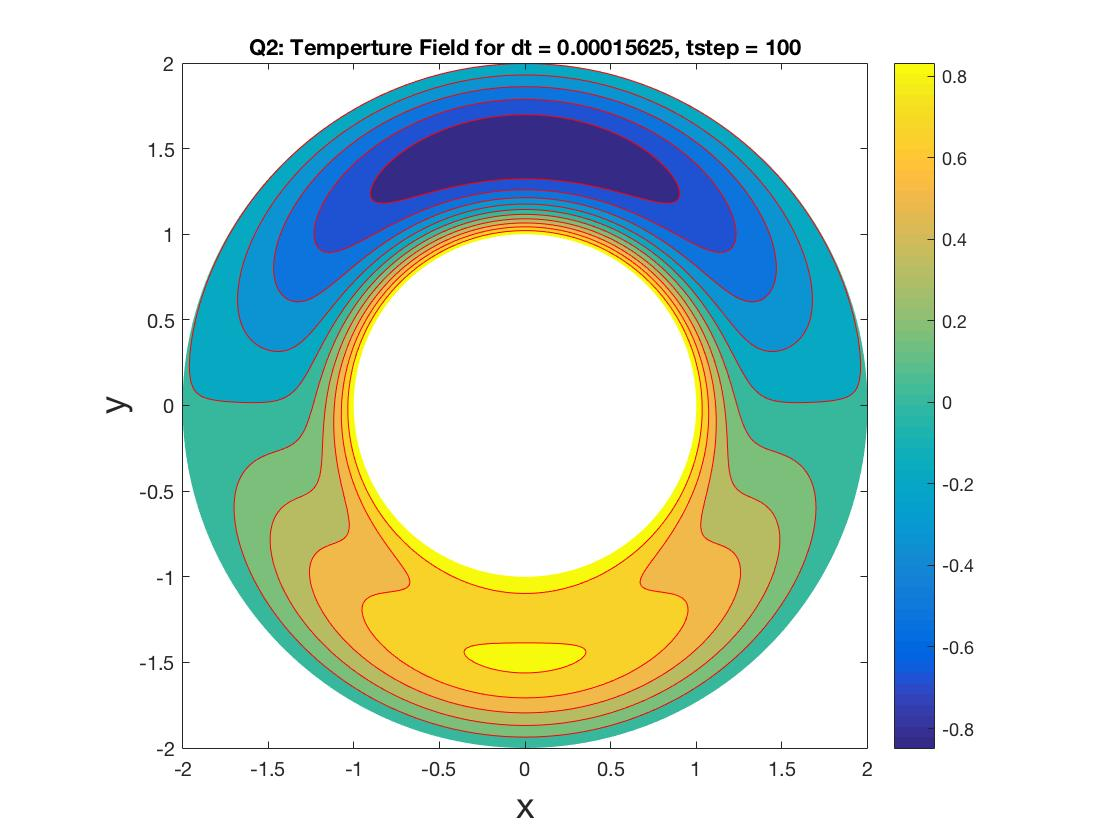
\includegraphics[width = 0.49\textwidth]{fig_q2DiffuseTest100}
		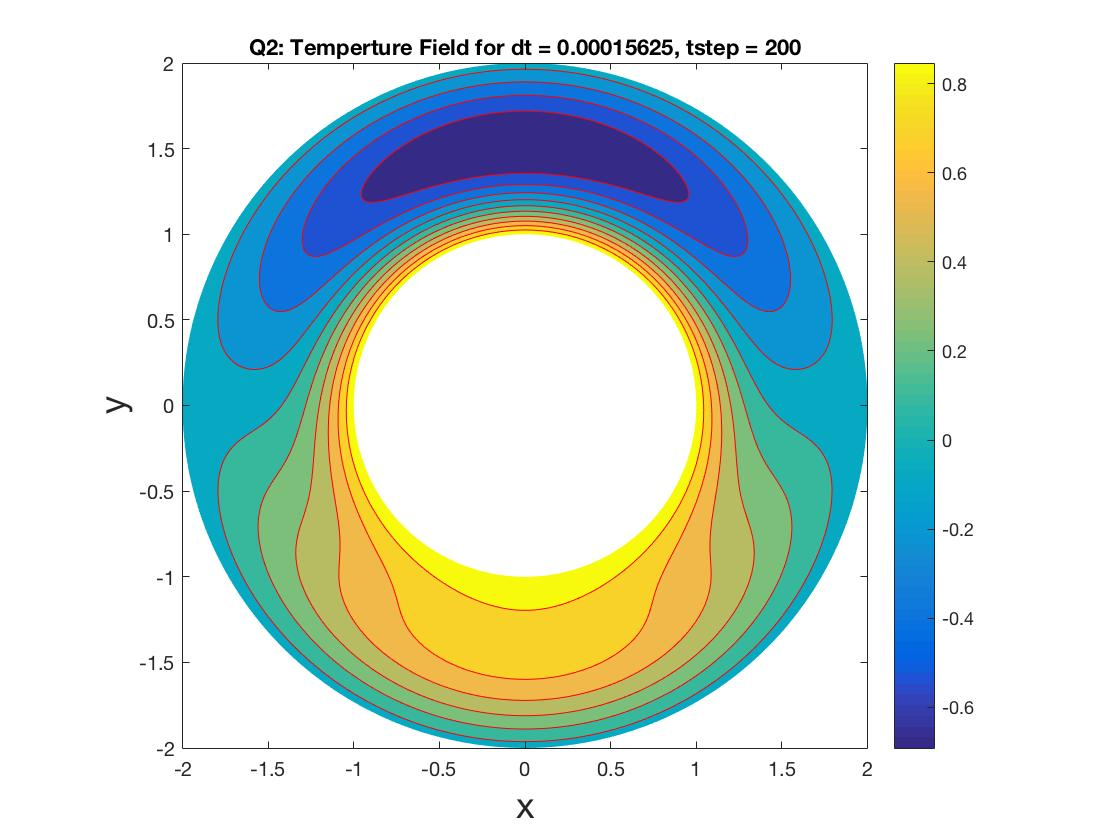
\includegraphics[width = 0.49\textwidth]{fig_q2DiffuseTest200}
		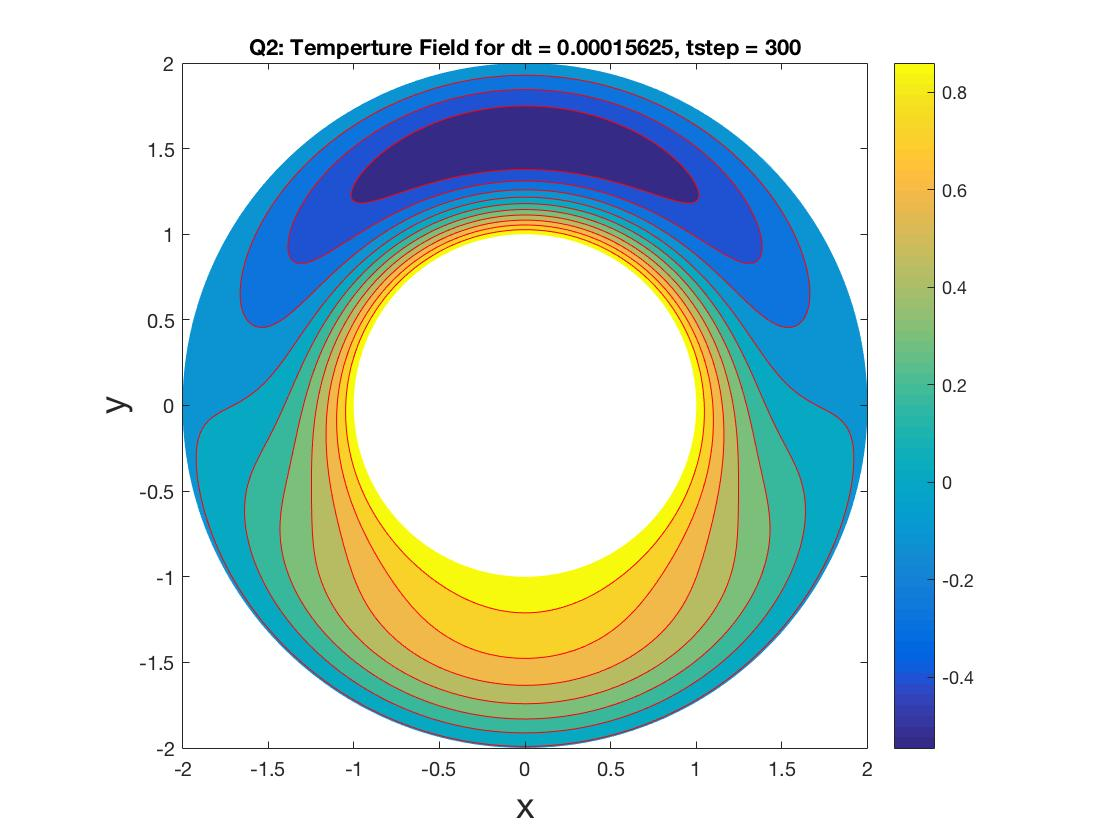
\includegraphics[width = 0.49\textwidth]{fig_q2DiffuseTest300}
		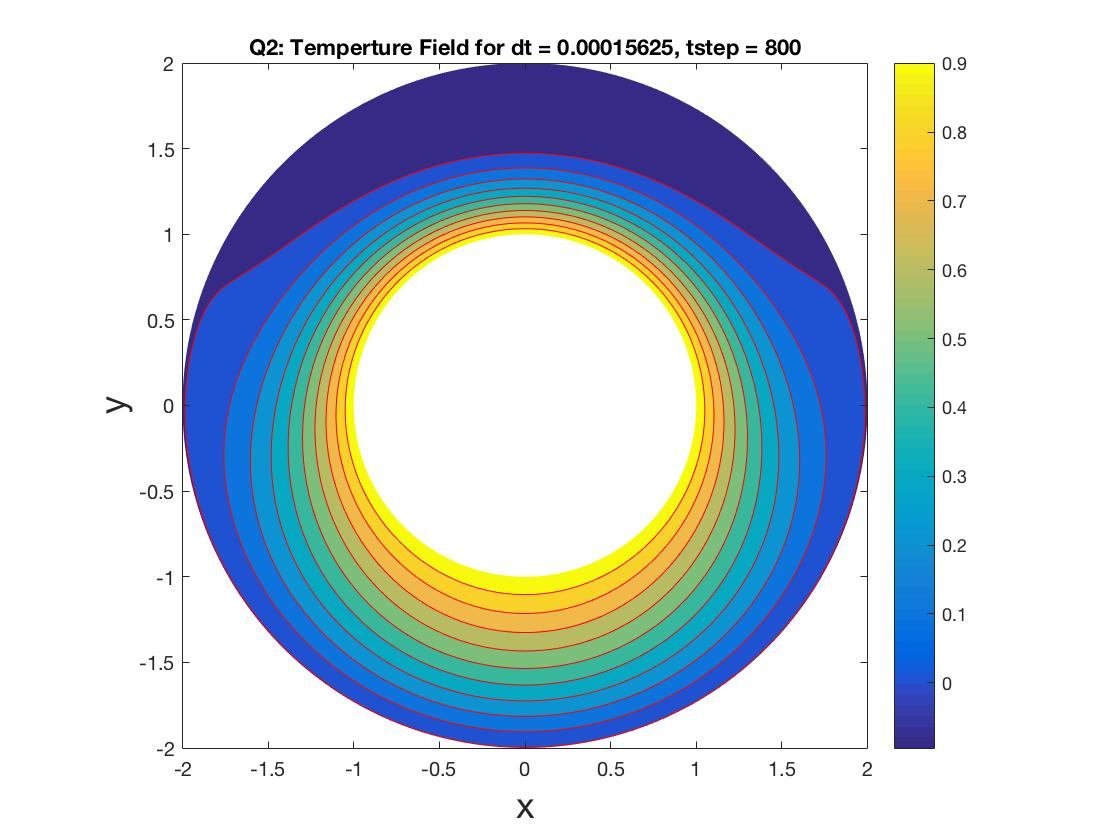
\includegraphics[width = 0.49\textwidth]{fig_q2DiffuseTest800}
		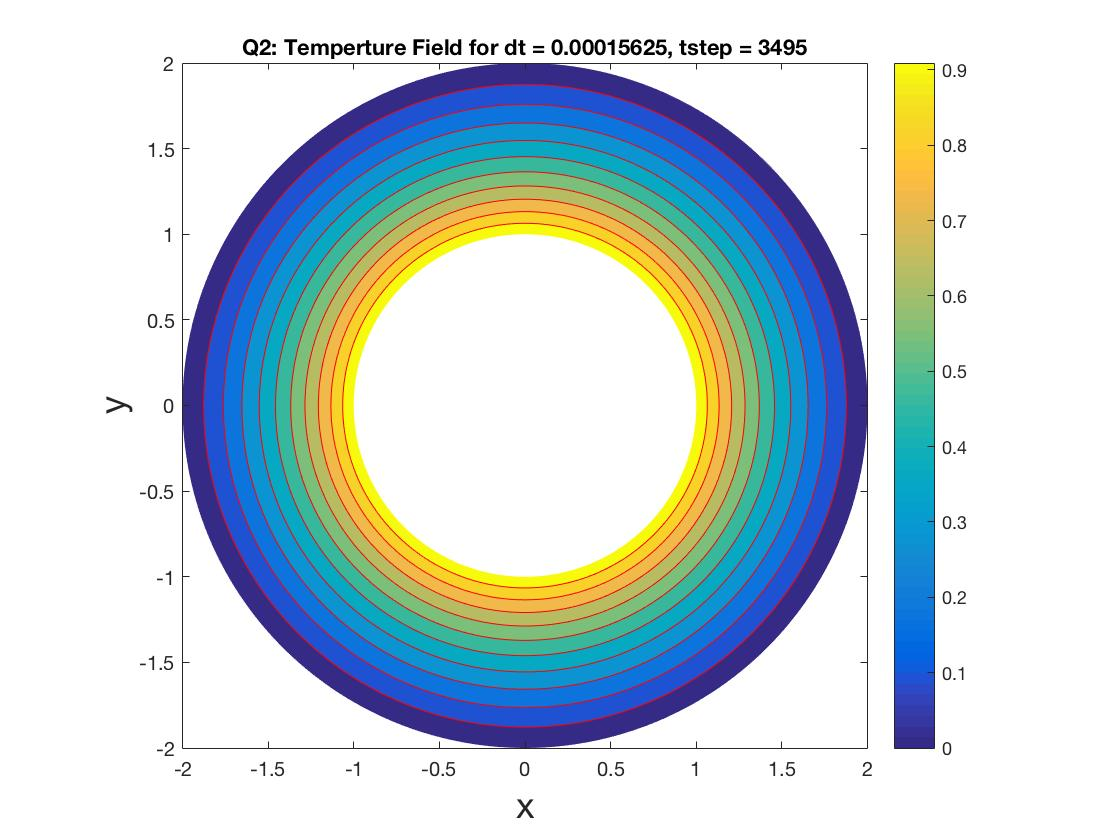
\includegraphics[width = 0.49\textwidth]{fig_q2DiffuseTest3495}
		\caption{Q2: Diffusing the specified field $Q_0$ for $\delta t = 1.5625e-04$ with $M = 2^6$ and $N=2^8$. The solution converges to a tolerance of $10^{-5}$ for the difference between the maximum error between iterations after 3495 iterations.}
		\label{fig:q2DiffuseTest}
	\end{figure}
	%%%%%%%%%%%%%%%%%%%%%%%%%%%%%%%%%%%%%%%%%%%%%%%%%%%%%%%%%%%%

\subsection{Combining Advection and Diffusion}

Now that we are happy with the functioning of the diffusion routine, it is combined with the advection routine to solve for the Temperature field in the annulus. This is done by trying solving the combined problem 
	
\begin{align}
	T_t + \textbf{u} \cdot \nabla T = \kappa \nabla^2 T
\end{align}

where $\kappa$ controls the rate of diffusion compared to that of advection. This equation is solved by first solving for $T_t = - \textbf{u} \cdot \nabla T$ and then $T_t = \kappa \nabla^2 T$.

In order to the test the impact of $kappa$ term, we have chosen the non-negative temperature field

\begin{align}
	T_0(r,\theta) =  \sin(\pi r)^2 \sin(\theta)^2 + \frac{r-b}{1-b}
	\label{eq:q2T0}
\end{align}

	%%%%%%%%%%%%%%%%%%%%%%%%%%%%%%%%%%%%%%%%%%%%%%%%%%%%%%%%%%%%
	\begin{figure}[h!]
		\centering
		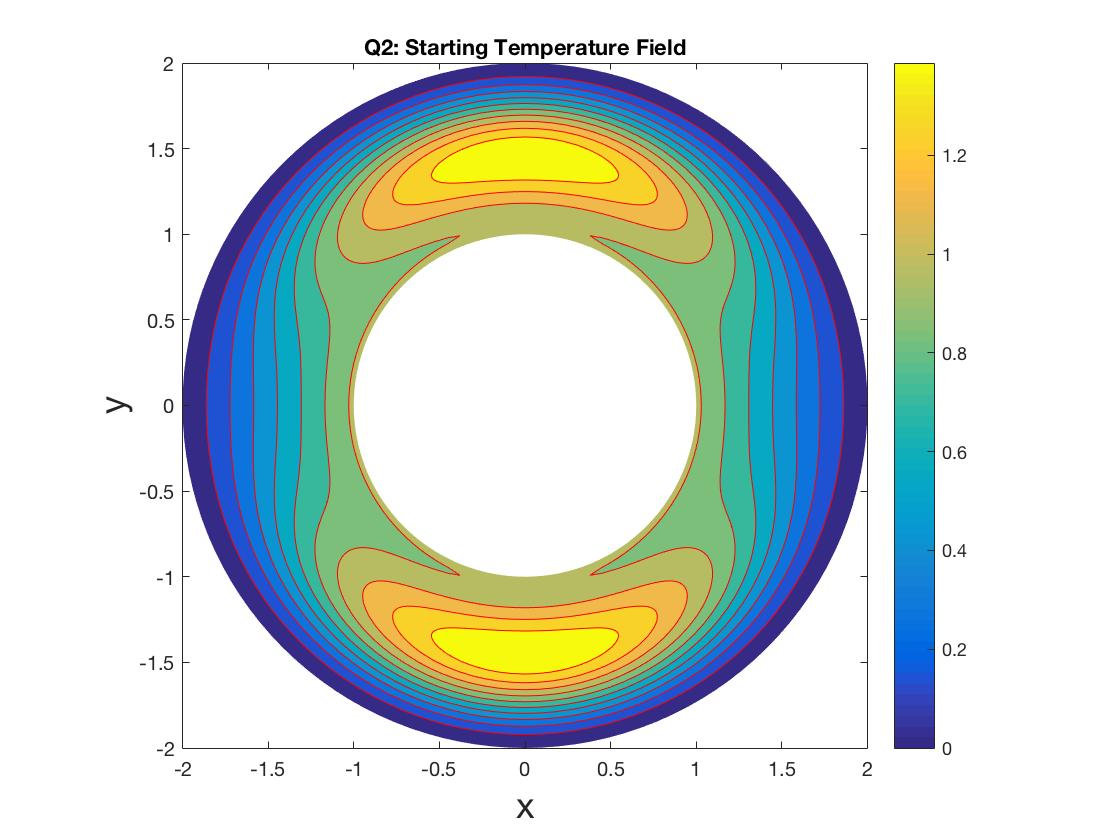
\includegraphics[width = 0.8\textwidth]{fig_q2KappaStart}
		\caption{Q2: Starting Temperature Field defined in Equation \ref{eq:q2T0} to test the impact of varying $\kappa$ with $M = 2^6$ and $N=2^8$.}
		\label{fig:q2KappaStart}
	\end{figure}
	%%%%%%%%%%%%%%%%%%%%%%%%%%%%%%%%%%%%%%%%%%%%%%%%%%%%%%%%%%%%

which obeys $T_0(1,:) = 1$ and $T_0(b,:) = 0$. The chosen stream function, $\psi$, is 

\begin{align}
	 \psi = (r - b)^2 (r - 1)^2  e^{ \sin(2 \theta) }
	 \label{eq:q2Psi}
\end{align}

which obeys $\psi = \psi_r = 0$ on $\partial \Omega$ and so we have a suitable velocity field.

	%%%%%%%%%%%%%%%%%%%%%%%%%%%%%%%%%%%%%%%%%%%%%%%%%%%%%%%%%%%%
	\begin{figure}[h!]
		\centering
		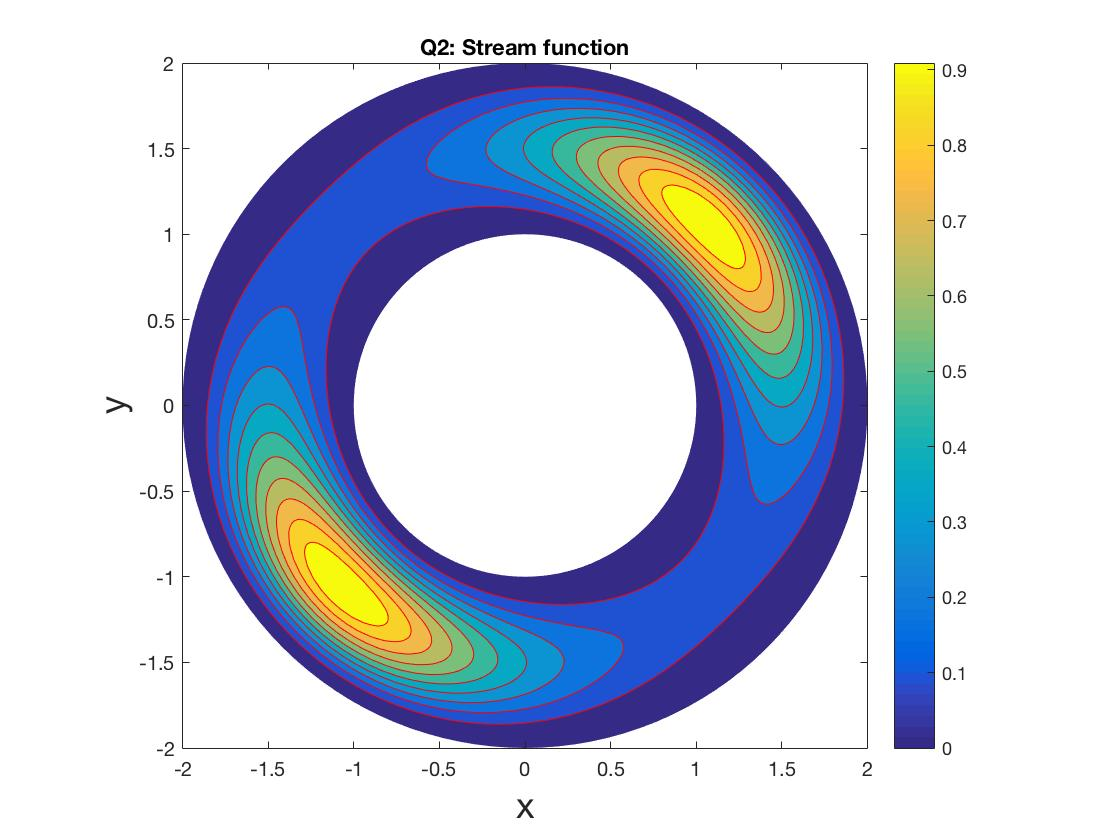
\includegraphics[width = 0.49\textwidth]{fig_q2psi}
		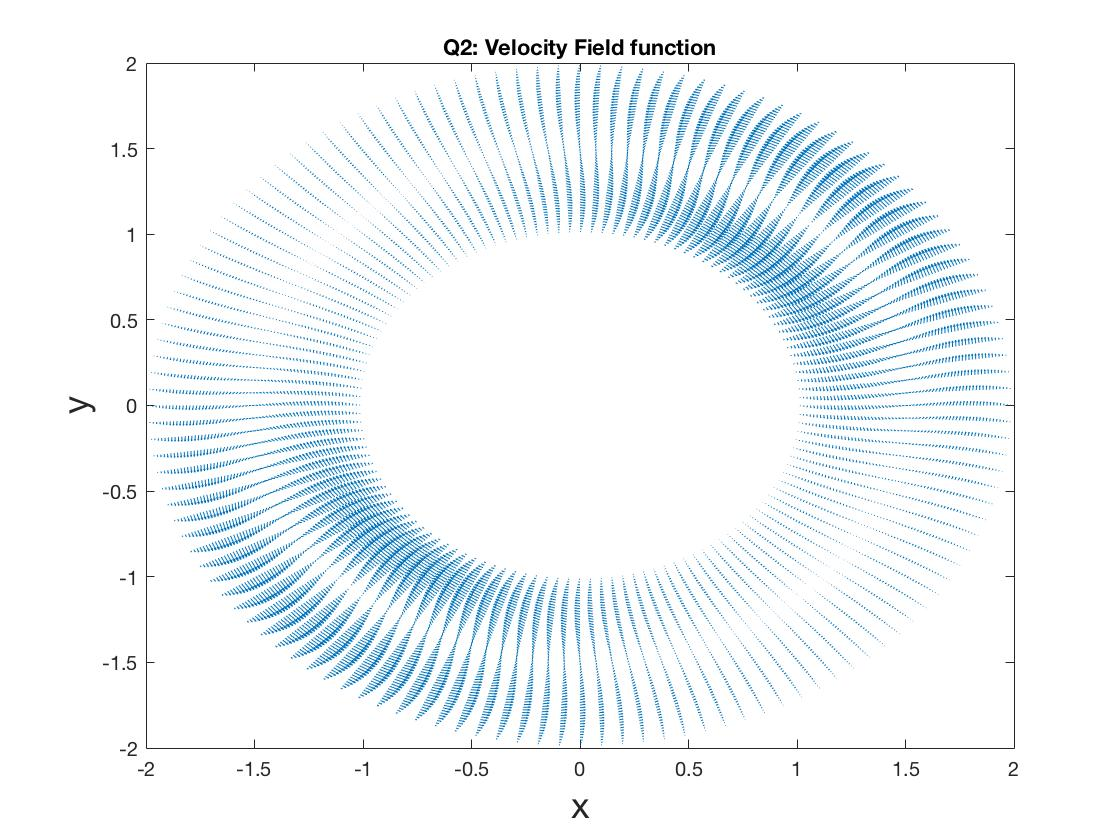
\includegraphics[width = 0.49\textwidth]{fig_q2ufield}
		\caption{Q2: Stream Function Field defined in Equation \ref{eq:q2Psi} to test the impact of varying $\kappa$ with $M = 2^6$ and $N=2^8$ along with the derived velocity field.}
		\label{fig:q2KappaPsi}
	\end{figure}
	%%%%%%%%%%%%%%%%%%%%%%%%%%%%%%%%%%%%%%%%%%%%%%%%%%%%%%%%%%%%

	%%%%%%%%%%%%%%%%%%%%%%%%%%%%%%%%%%%%%%%%%%%%%%%%%%%%%%%%%%%%
	\begin{figure}[h!]
		\centering
		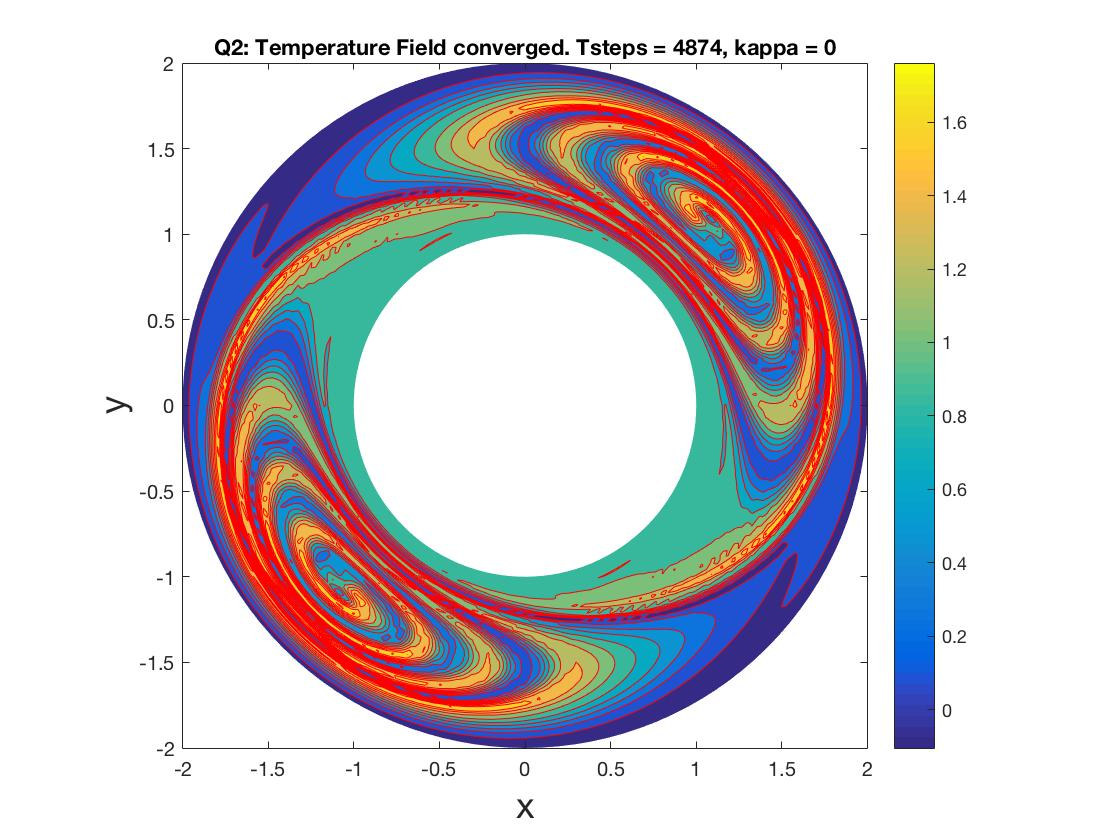
\includegraphics[width = 0.49\textwidth]{fig_q2Kappa0}
		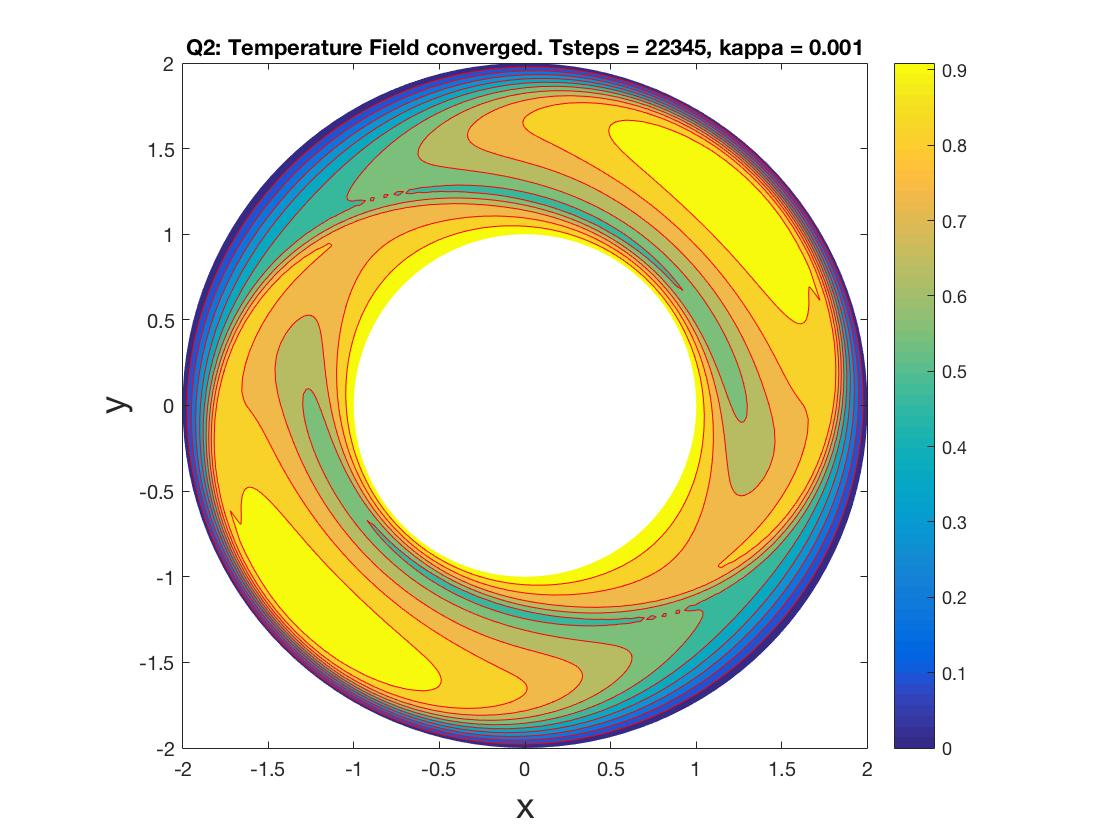
\includegraphics[width = 0.49\textwidth]{fig_q2Kappa0001}
		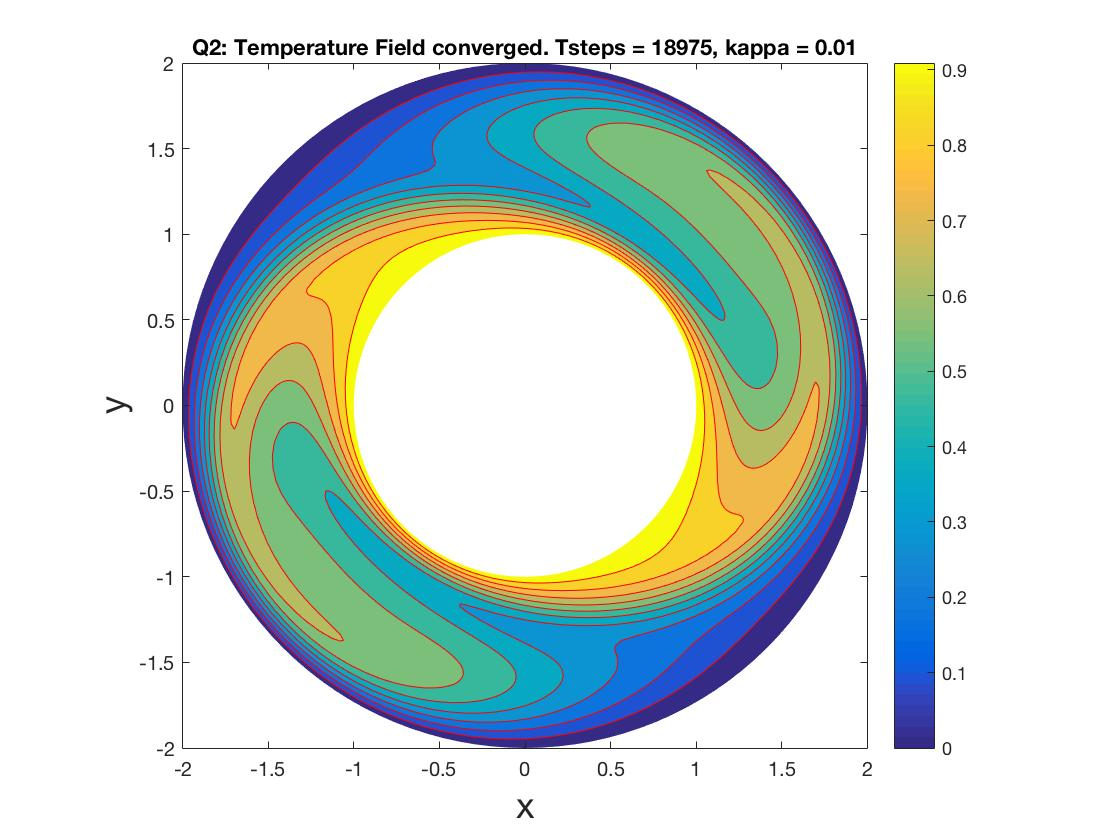
\includegraphics[width = 0.49\textwidth]{fig_q2Kappa001}
		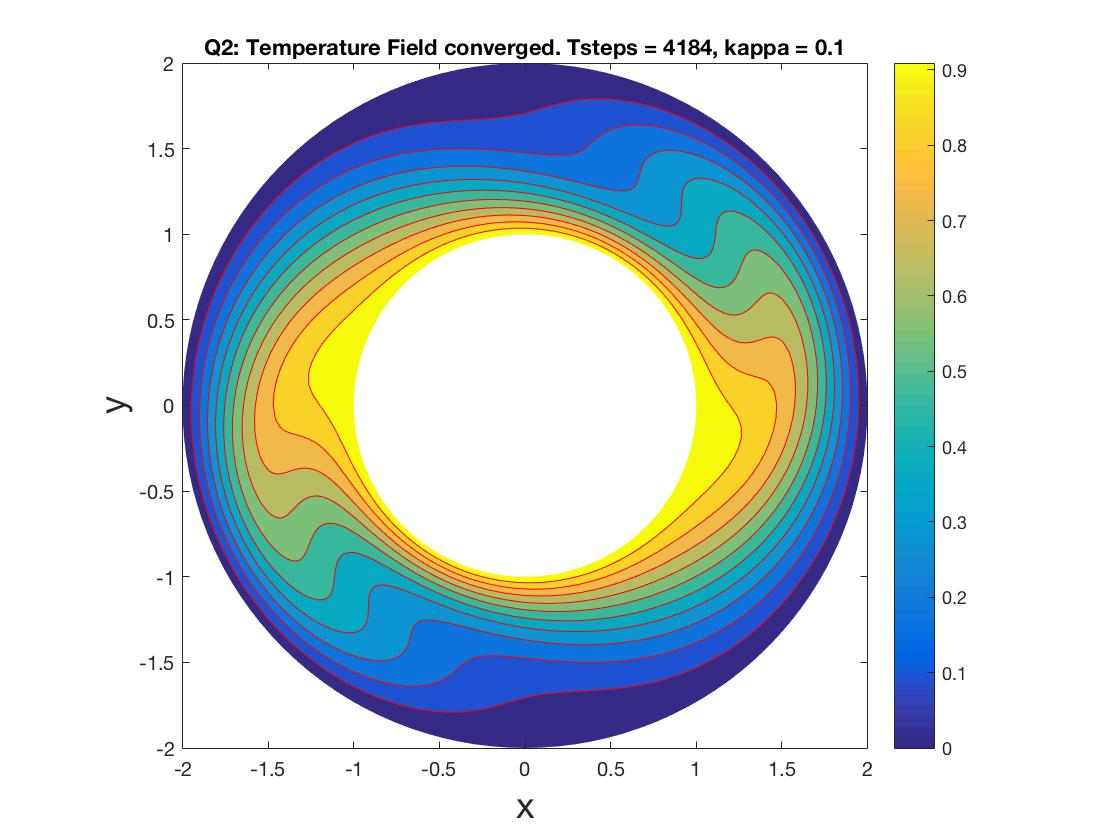
\includegraphics[width = 0.49\textwidth]{fig_q2Kappa01}
		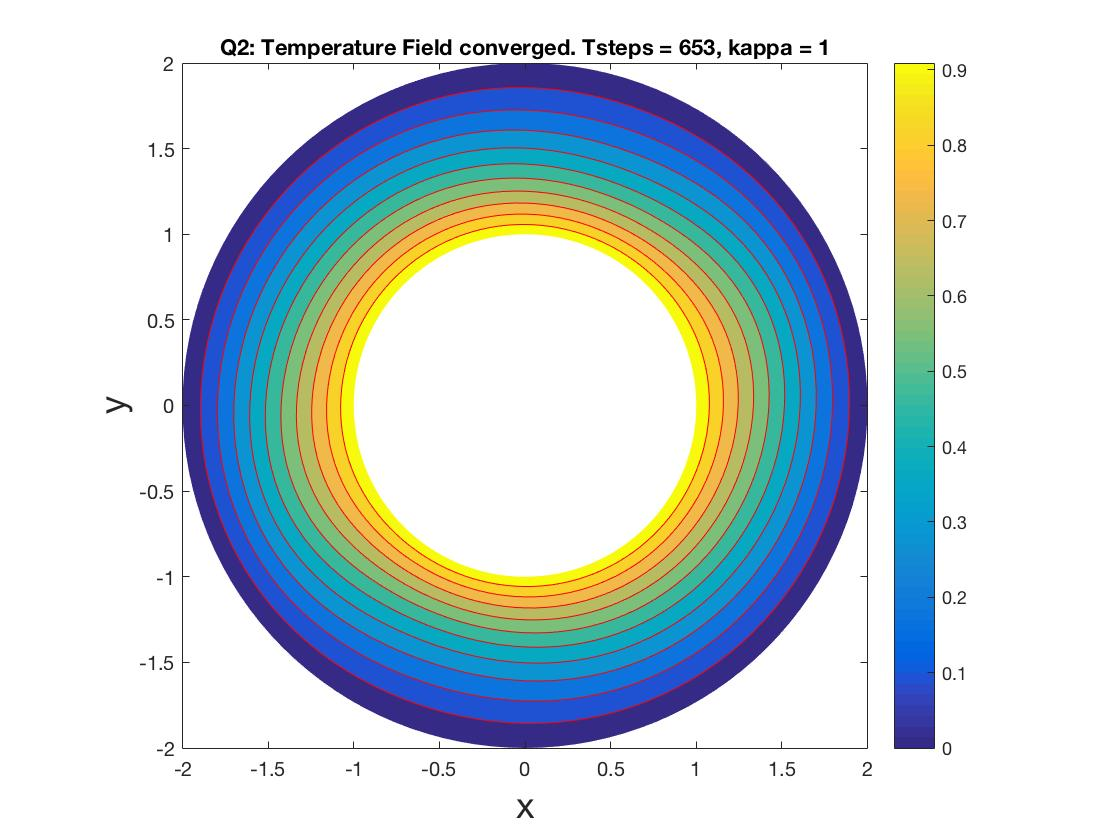
\includegraphics[width = 0.49\textwidth]{fig_q2Kappa1}
		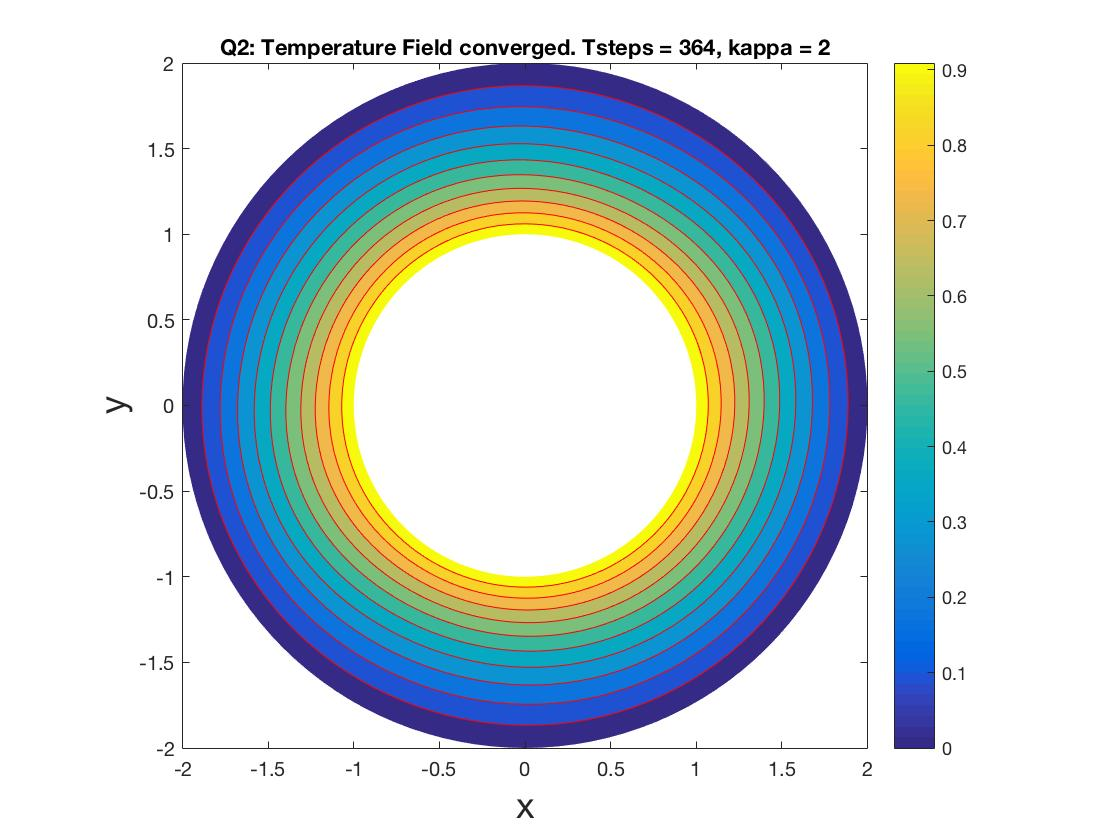
\includegraphics[width = 0.49\textwidth]{fig_q2Kappa2}
		\caption{Q2: Advecting and Diffusing the specified field $T_0$ for $\delta t = 1e-03$ with $M = 2^6$ and $N=2^8$. Iterations are stopped when the maximum difference between subsequent $T$'s converges to a tolerance of $10^{-5}$.}
		\label{fig:q2Kappa}
	\end{figure}
	%%%%%%%%%%%%%%%%%%%%%%%%%%%%%%%%%%%%%%%%%%%%%%%%%%%%%%%%%%%%

Figure \ref{fig:q2Kappa} shows the results of the varying $\kappa$ on advection-diffusion routine. These results are derived by varying the value of $\kappa$ in \texttt{q2.m}. $\kappa = 0$ gives a purely advected solution. This created large gradients as the Temperature is advected around the swirls without diffusing at all. $\kappa = 0.001$ mimics the pure advection solution closely but with the large gradients in the Temperature smoothed out. As $\kappa$ is increased, the solution starts to become more uniform. For $\kappa=1$ the solution is an almost uniform (i.e. the pure diffusion solution) but with slight bulges due to to velocity field. For $\kappa = 2$ the solution looks almost identical to the pure diffusion linear gradient solution. In terms the number of iterations to converge, as $\kappa \rightarrow 0$ the number of iterations $\rightarrow \infty$. For $\kappa = 0$, the solution never converges (for the given definition) as it keeps on advecting. This is reasonable as for larger $\kappa$ there is greater diffusion and the field becomes more uniform more quickly. 

%%%%%%%%%%%%%%%%%%%%%%%%%%%%%%%%%%%%%%%%%%%%%%%%%%%%%%%%%%%%
\section{Vorticity}

The vorticity equation is

\begin{align}
	\omega_t + \textbf{u} \cdot \nabla \omega = \nabla^2 \omega + F
\end{align}

where $F$ is some forcing. The Dirichlet conditions on $\psi$ are $\psi = 0$ on $\partial \Omega$. 

The Dirichlet condition for $\omega$ is slightly more complicated. We know that $\psi_r = 0$ on $\partial \Omega$. Starting from 

\begin{align*}
	-\omega &= \nabla^2 \psi \\
	\omega &= -\psi_{rr} - \frac{1}{3}\psi_r - \frac{1}{r^2}\psi_{\theta \theta}
\end{align*}

Since $\psi = 0$ on $\partial \Omega$ then so does $\psi_\theta$ and $\psi_{\theta \theta}$. Thus we can further simplify to

\begin{align*}
	\omega = -\psi_{rr}
\end{align*}

This can now we solved using the same method as in Lecture 20 by taking a Taylor expansion $\psi$ around the boundaries, eliminating known terms, estimating the unknown term and finally getting individual Dirichlet conditions on each boundary. This has been implemented in \texttt{omega\_BC.m}. 

So now to solve the vorticity equation, we do exactly as was done in Question 2 where we first advect the field and then diffuse it. Since advection does not change the values on $\partial \Omega$, it can be used without any alterations for this too. For the diffusion routine, a simple alteration of enforcing the non-zero Dirichlet boundary condition is added. This code can be found in \texttt{omega\_MultiGridV.m}, \texttt{omega\_GaussSeidel.m} and \texttt{omega\_residual.m}.

In order to test the complete routine, we use the same function (Equation \ref{eq:q2T0}) as for testing the advection-diffusion routine in the previous section. Further we  have chosen a forcing function, $F$, same as Equation \ref{eq:T1}.

This has been implemented in \texttt{q3.m} that utilizes \texttt{psi\_Eqn.m}, \texttt{psi\_MultiGridV.m}, \texttt{psi\_GaussSeidel.m} and \texttt{psi\_residual.m}. The solution is considered converged once the maximum difference between errors is less than $10^{-10}$. The results can be seen in Figure \ref{fig:q3} along with Figure \ref{fig:q1Advect} for the initial $\omega$. The routine appears to be working correctly as the computed final stream function, $\psi$, resembles the forcing function, $F$, closely. Changing the initial $\omega$ to within reason results in this final same solution and can be done by changing the code in \texttt{q3.m}.
	%%%%%%%%%%%%%%%%%%%%%%%%%%%%%%%%%%%%%%%%%%%%%%%%%%%%%%%%%%%%
	\begin{figure}[h!]
		\centering
		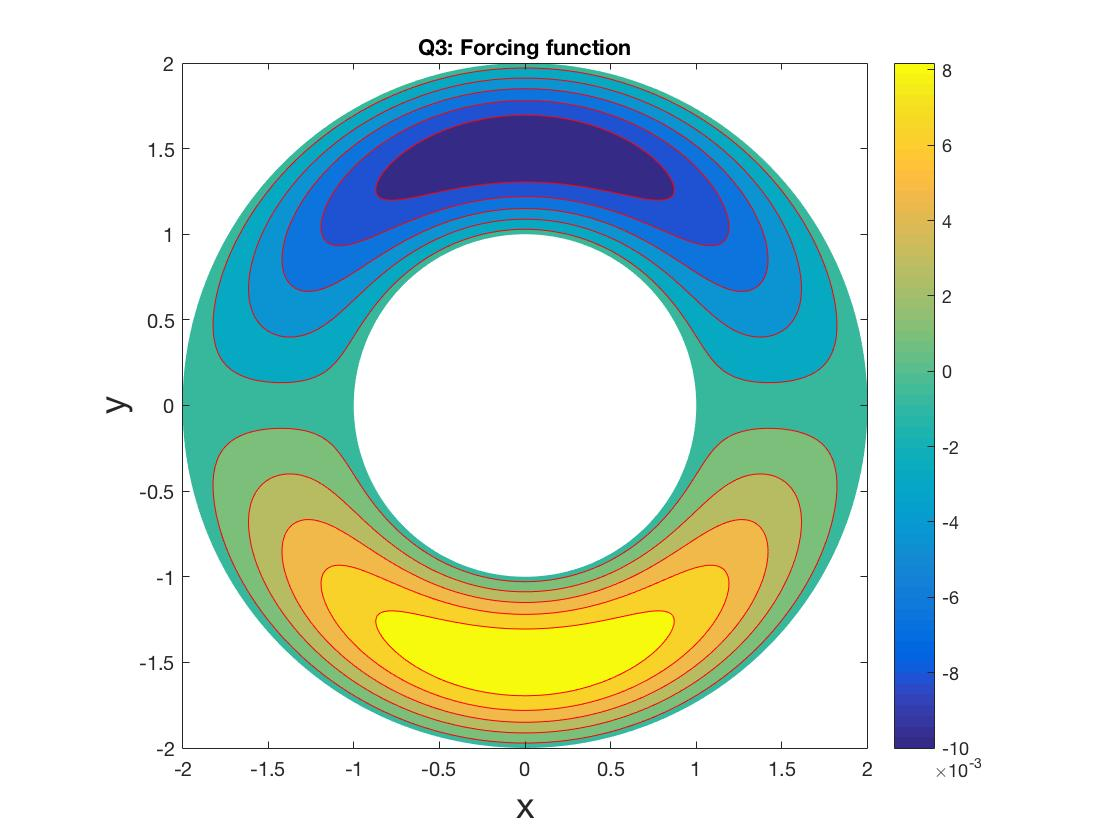
\includegraphics[width = 0.49\textwidth]{fig_q3F}
		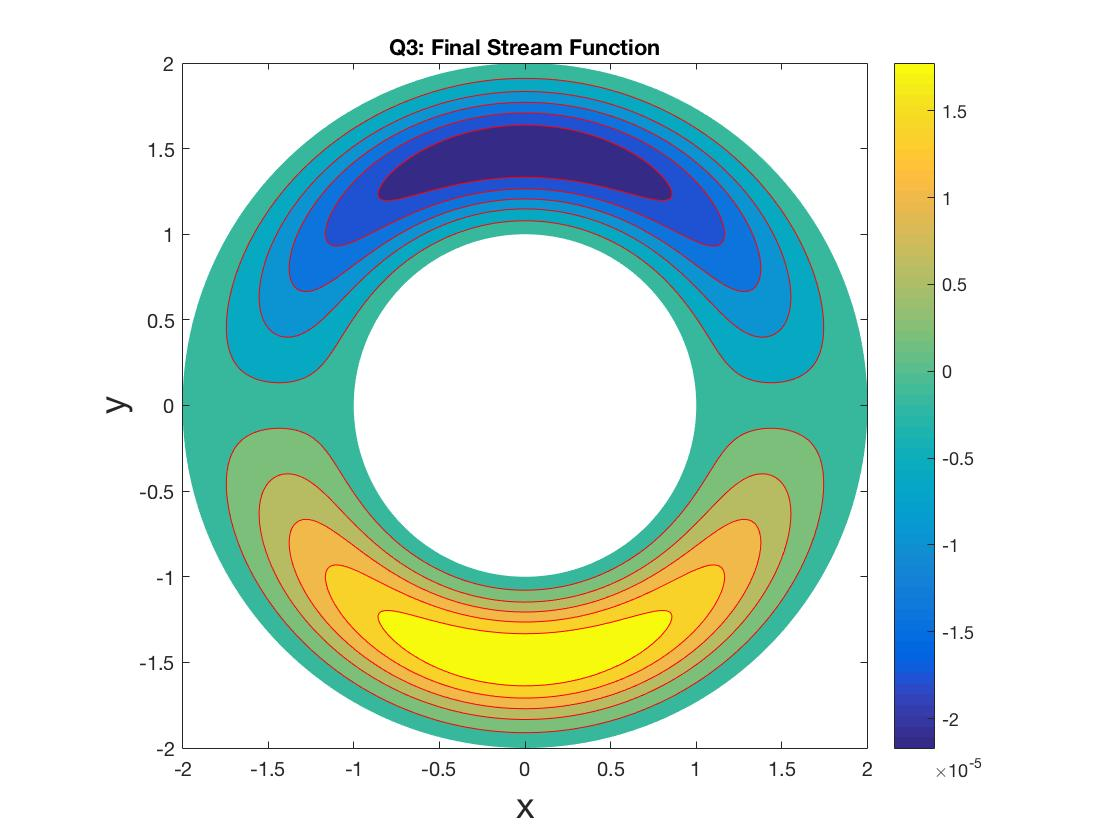
\includegraphics[width = 0.49\textwidth]{fig_q3psi}
		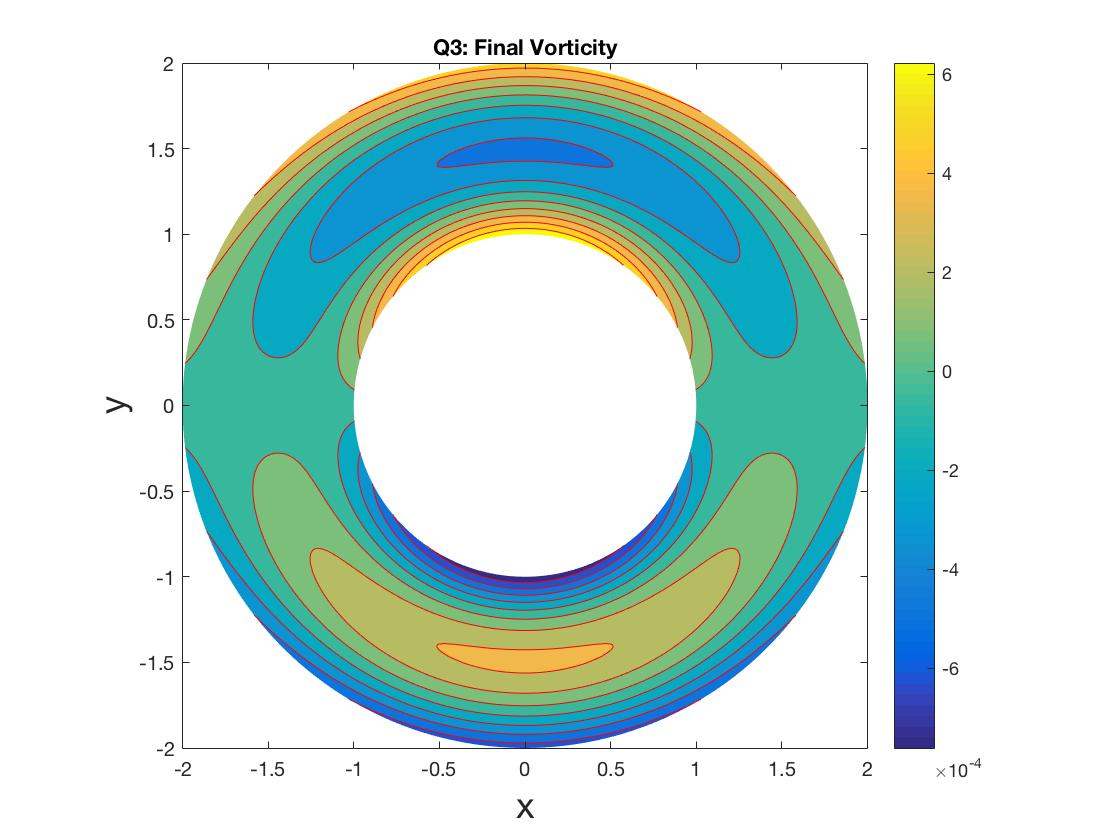
\includegraphics[width = 0.49\textwidth]{fig_q3omega}
		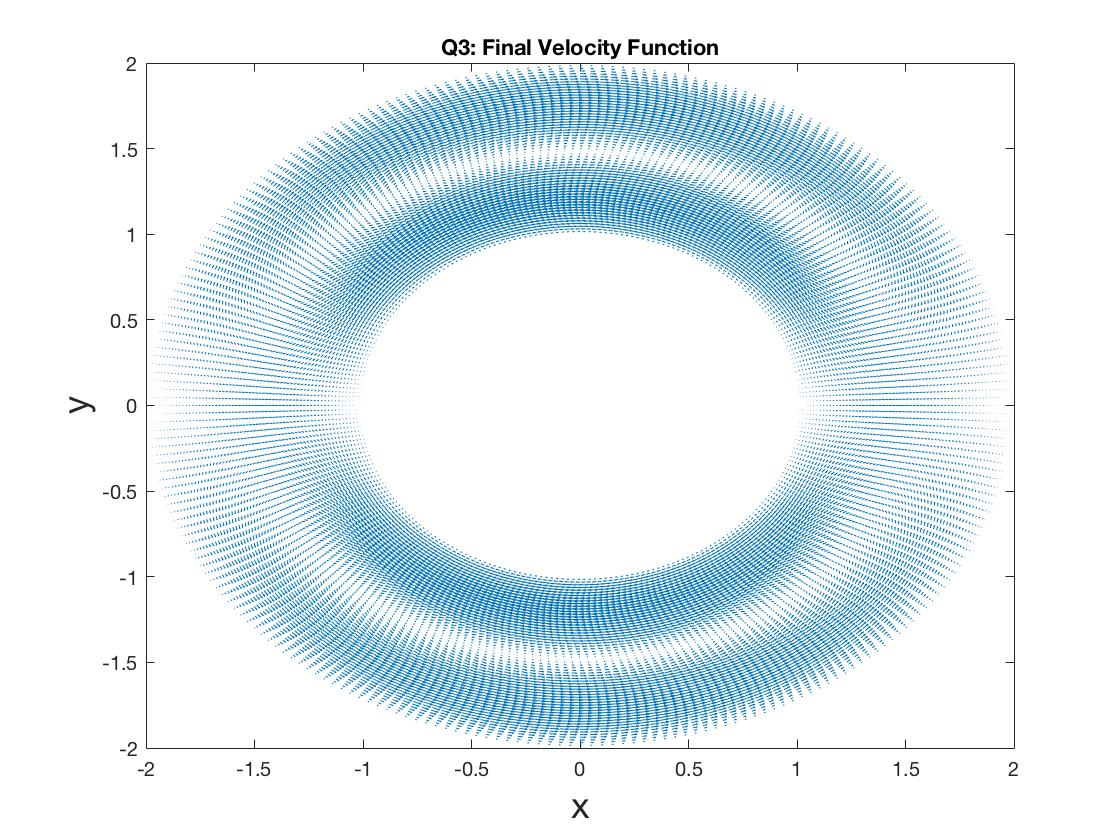
\includegraphics[width = 0.49\textwidth]{fig_q3u}
		\caption{Q3: Advecting and Diffusing the vorticity with $M = 2^6$ and $N=2^8$. Iterations are stopped when the maximum difference between subsequent $T$'s converges to a tolerance of $10^{-10}$.}
		\label{fig:q3}
	\end{figure}
	%%%%%%%%%%%%%%%%%%%%%%%%%%%%%%%%%%%%%%%%%%%%%%%%%%%%%%%%%%%%

%%%%%%%%%%%%%%%%%%%%%%%%%%%%%%%%%%%%%%%%%%%%%%%%%%%%%%%%%%%%
\section{The Full Problem}

Now that we can confident that the Advection-Diffusion routines are working properly for the Temperature as well as routines for solving the vorticity equation and finding $\psi$ from $\omega$, we can tackle the full problem. This has be done in \texttt{q4.m}. The main difference in the codes in the inclusion of 2 parameters: Rayleigh number and Prandtl number. The Rayleigh number, $R_a$, is a measure of the thermal driving force. The Prandtl number, $P_r$ is the ratio of the fluid kinematic viscosity to the thermal diffusivity which basically serves the same function as $\kappa$ for the Temperature field. Noting that the solution must be studied for various values of $b$ and various values of $\kappa$ as well this means that the parameter space we are interested in exploring is 4 dimension. This is obviously quite large and thus will not be exhaustively studied. Furthermore, we will stick to assessing situations arising from our specific perturbations.

We use a perturbation of 

\begin{align}
	T_0(r,\theta) &= 0.01 \left[ \sin(\pi r)^2 \sin(\theta)^2 + \frac{r-b}{1-b} \right] \\
	T_0(1,\theta) &= 1
\end{align}

throughout this section.

Firstly, we go about computing the mentioned $R_c$ value in the assignment.

\subsection{Approximate Value of $R_c$}

In this section it is assumed $\kappa = P_r = 1$ and $b=2$ to begin with.

This gives an approximation for $R_a \approx 3000$. This can be seen in Figure \ref{fig:q4Rab2}. Furthermore it seems that for larger values of $R_a$, the rolls appear to be closer to the $r=b$ boundary. I.e. they are in a sense stronger which makes sense with the given definition of the Rayleigh number being the thermal driving force as a stronger thermal driving force will result in stronger advection currents due to the perturbations in the temperature. For $b=2$, it seems that the varying the value of $R_a$ does not impact the number of rolls that appear as there are still 4 rolls for $R_a = 10000$. 

	%%%%%%%%%%%%%%%%%%%%%%%%%%%%%%%%%%%%%%%%%%%%%%%%%%%%%%%%%%%%
	\begin{figure}[h!]
		\centering
		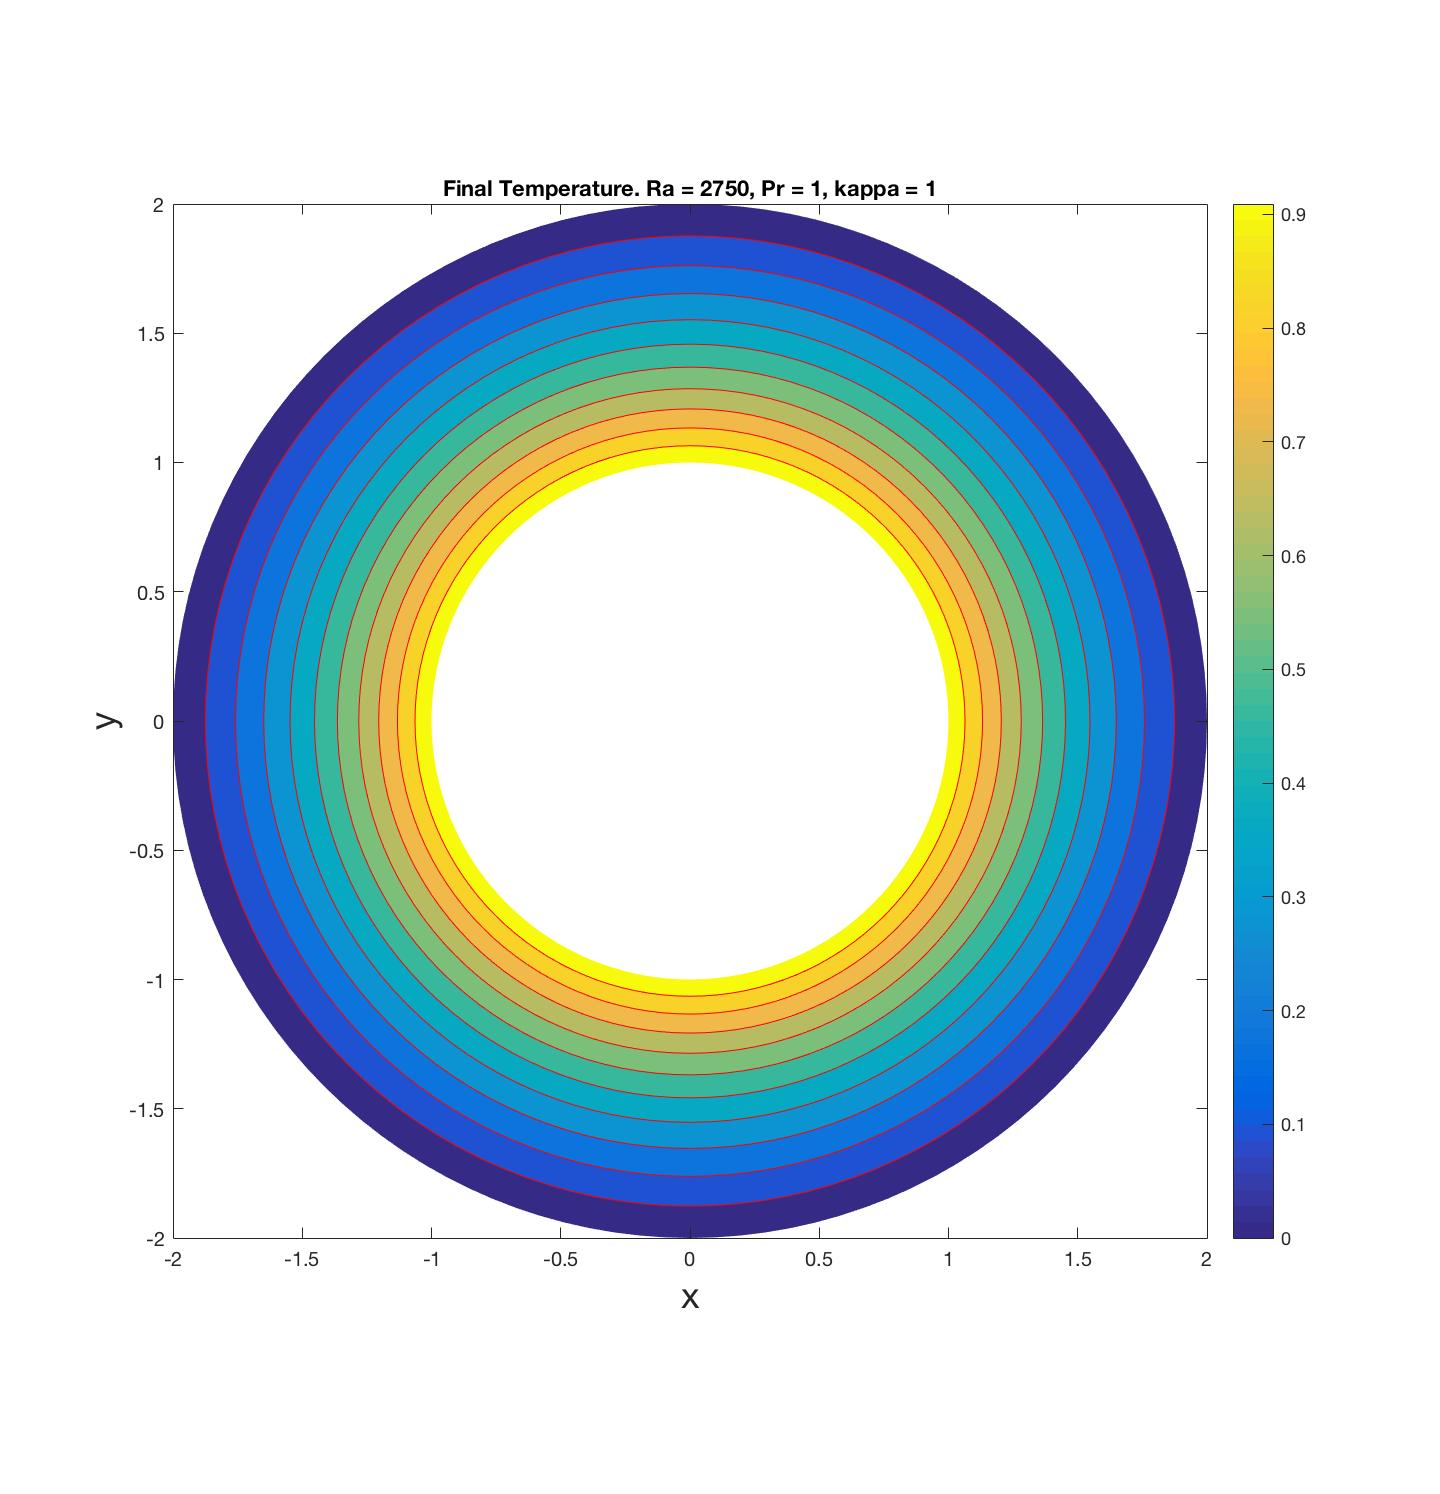
\includegraphics[width = 0.49\textwidth]{fig_q4ra2750}
		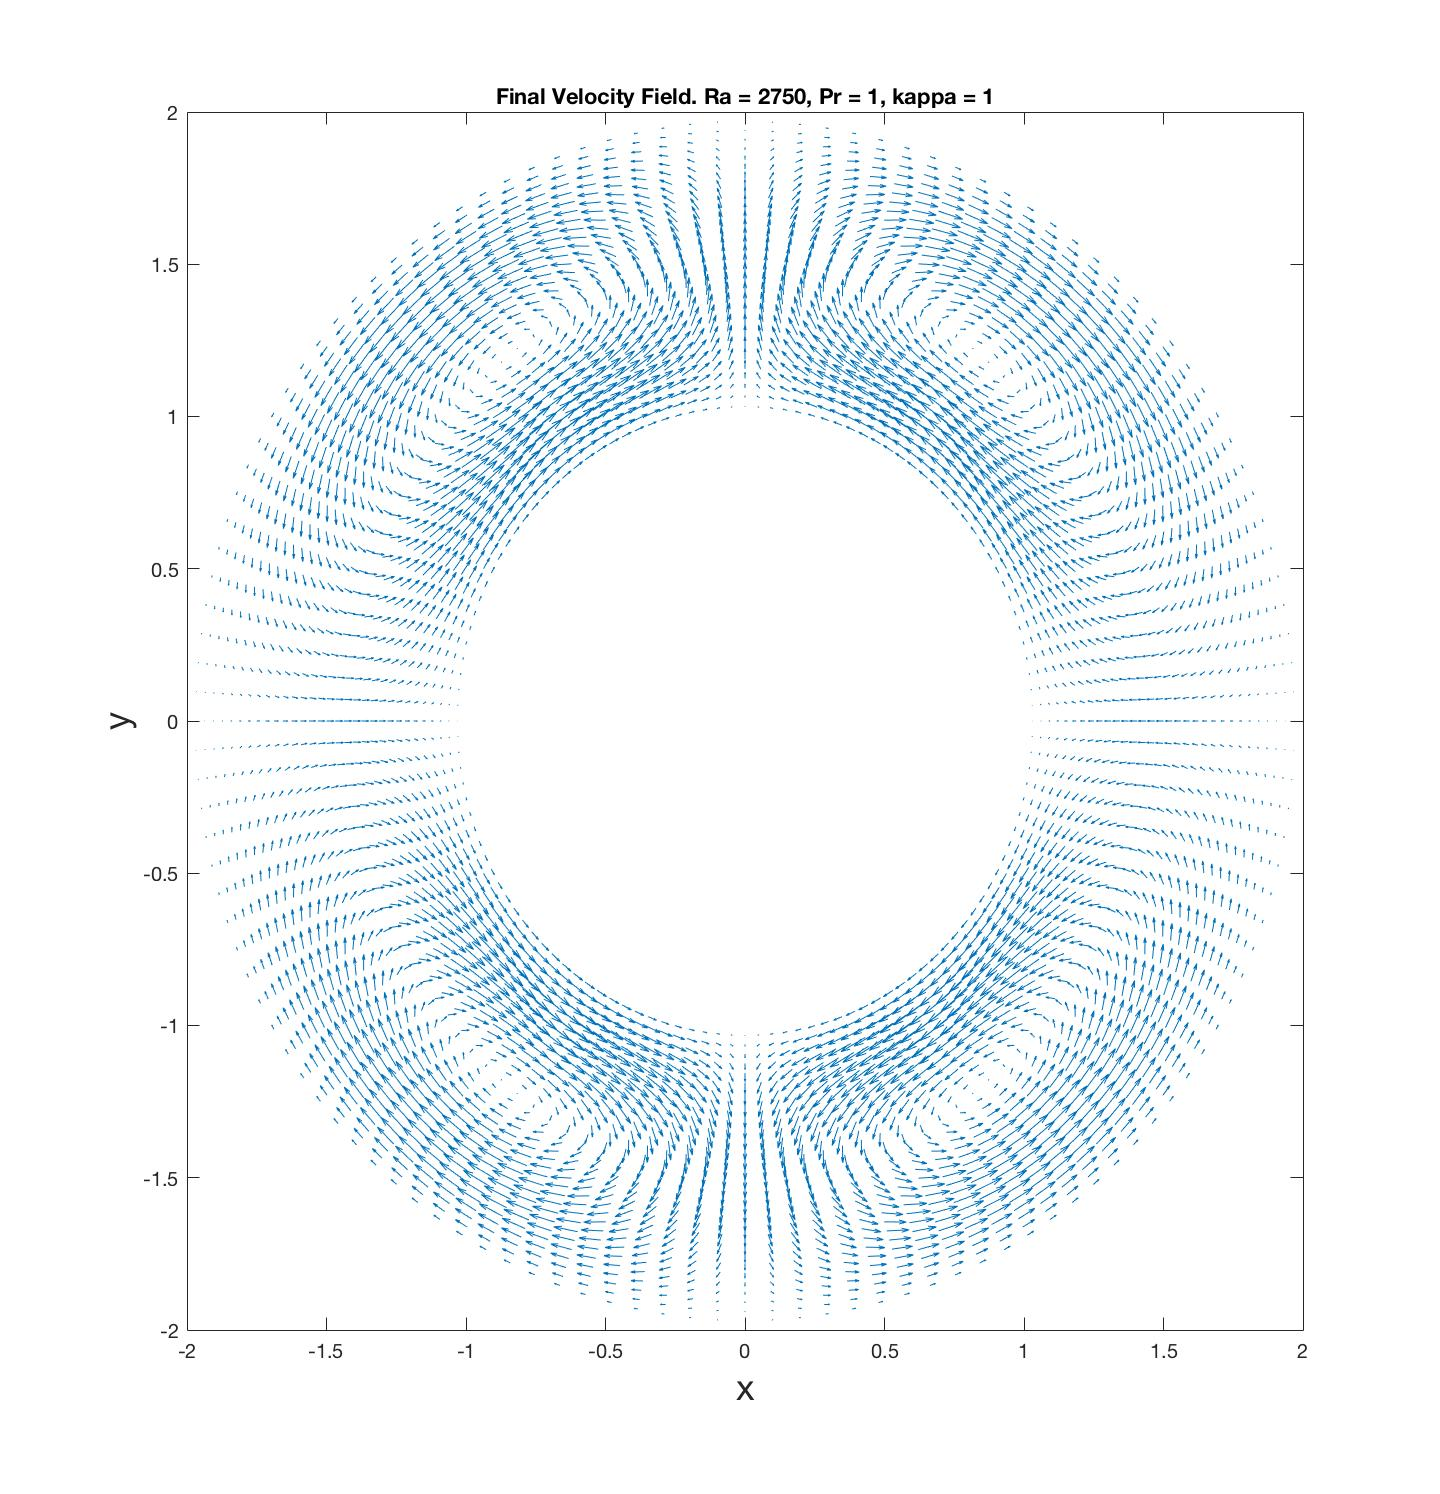
\includegraphics[width = 0.49\textwidth]{fig_q4ura2750}
		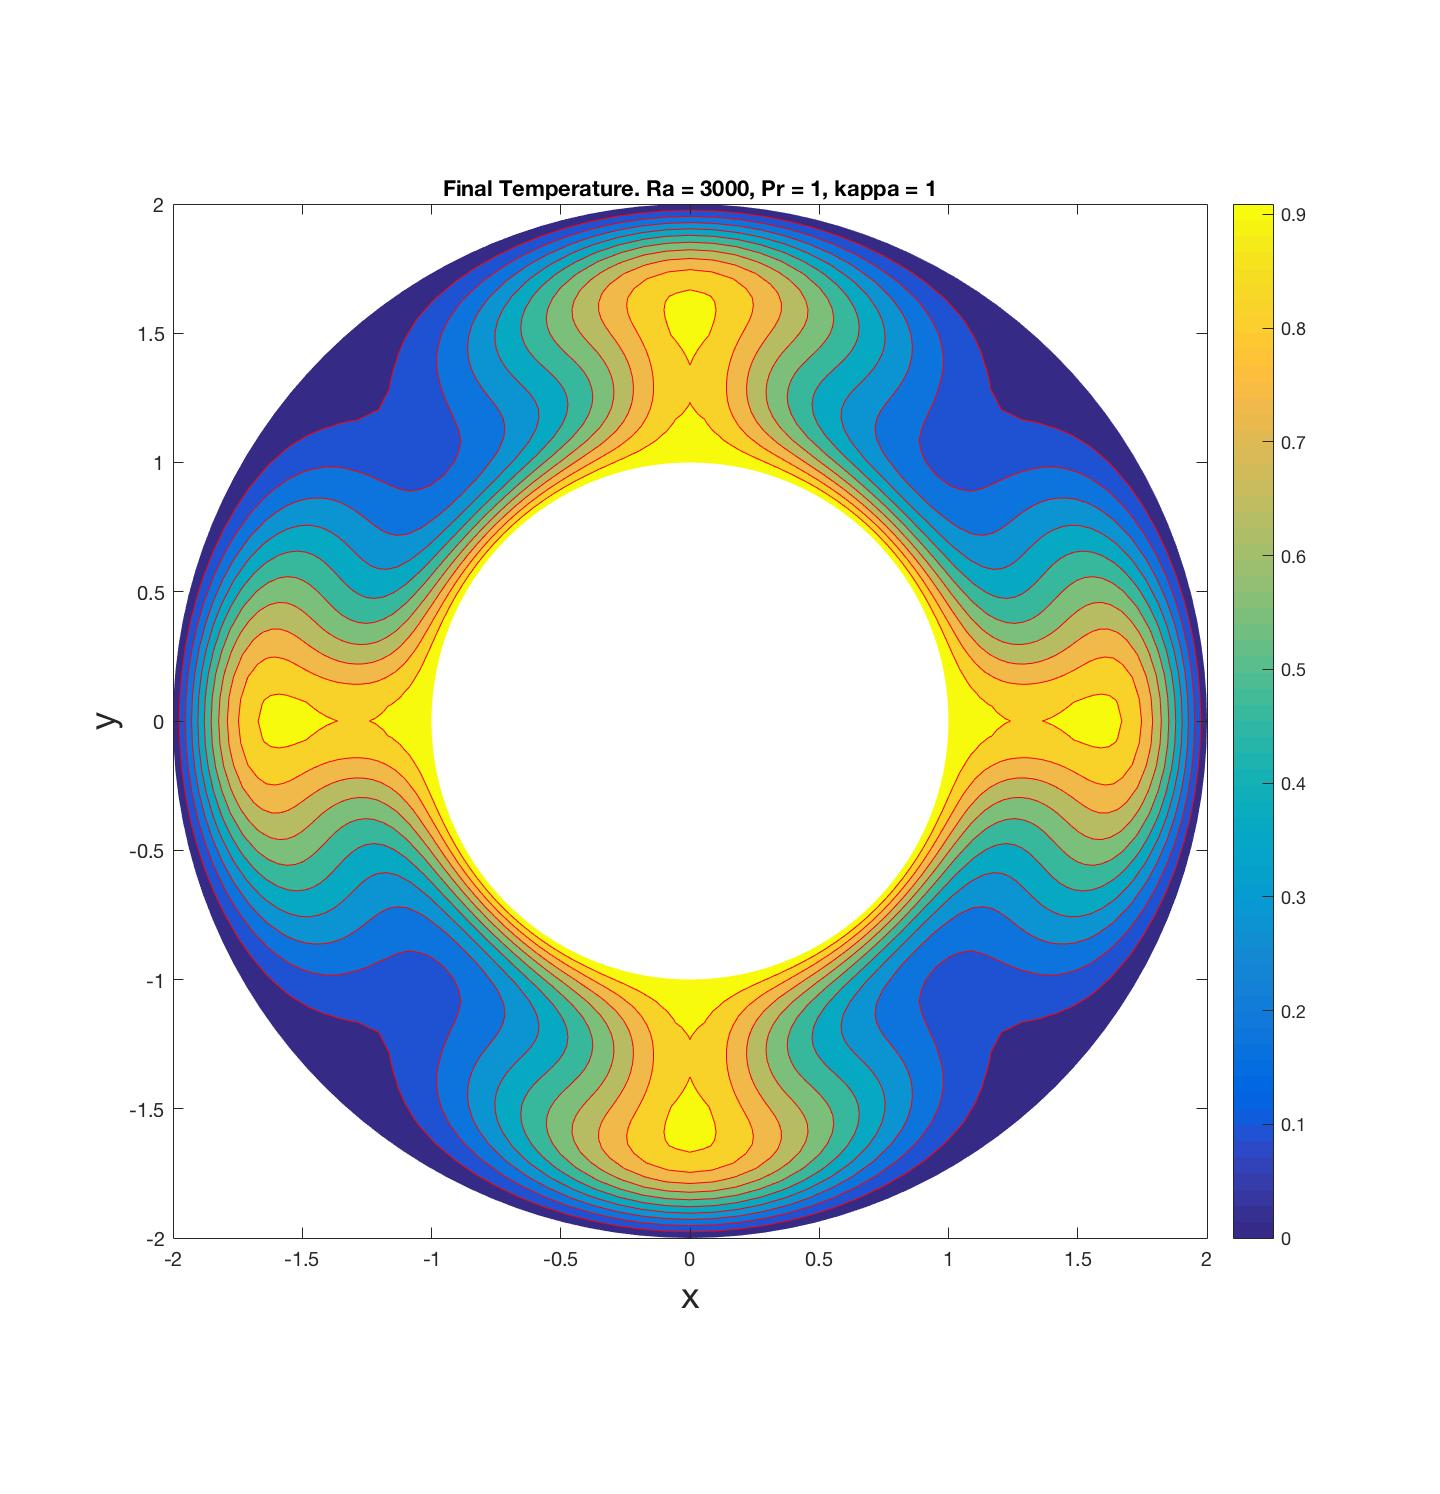
\includegraphics[width = 0.49\textwidth]{fig_q4ra3000}
		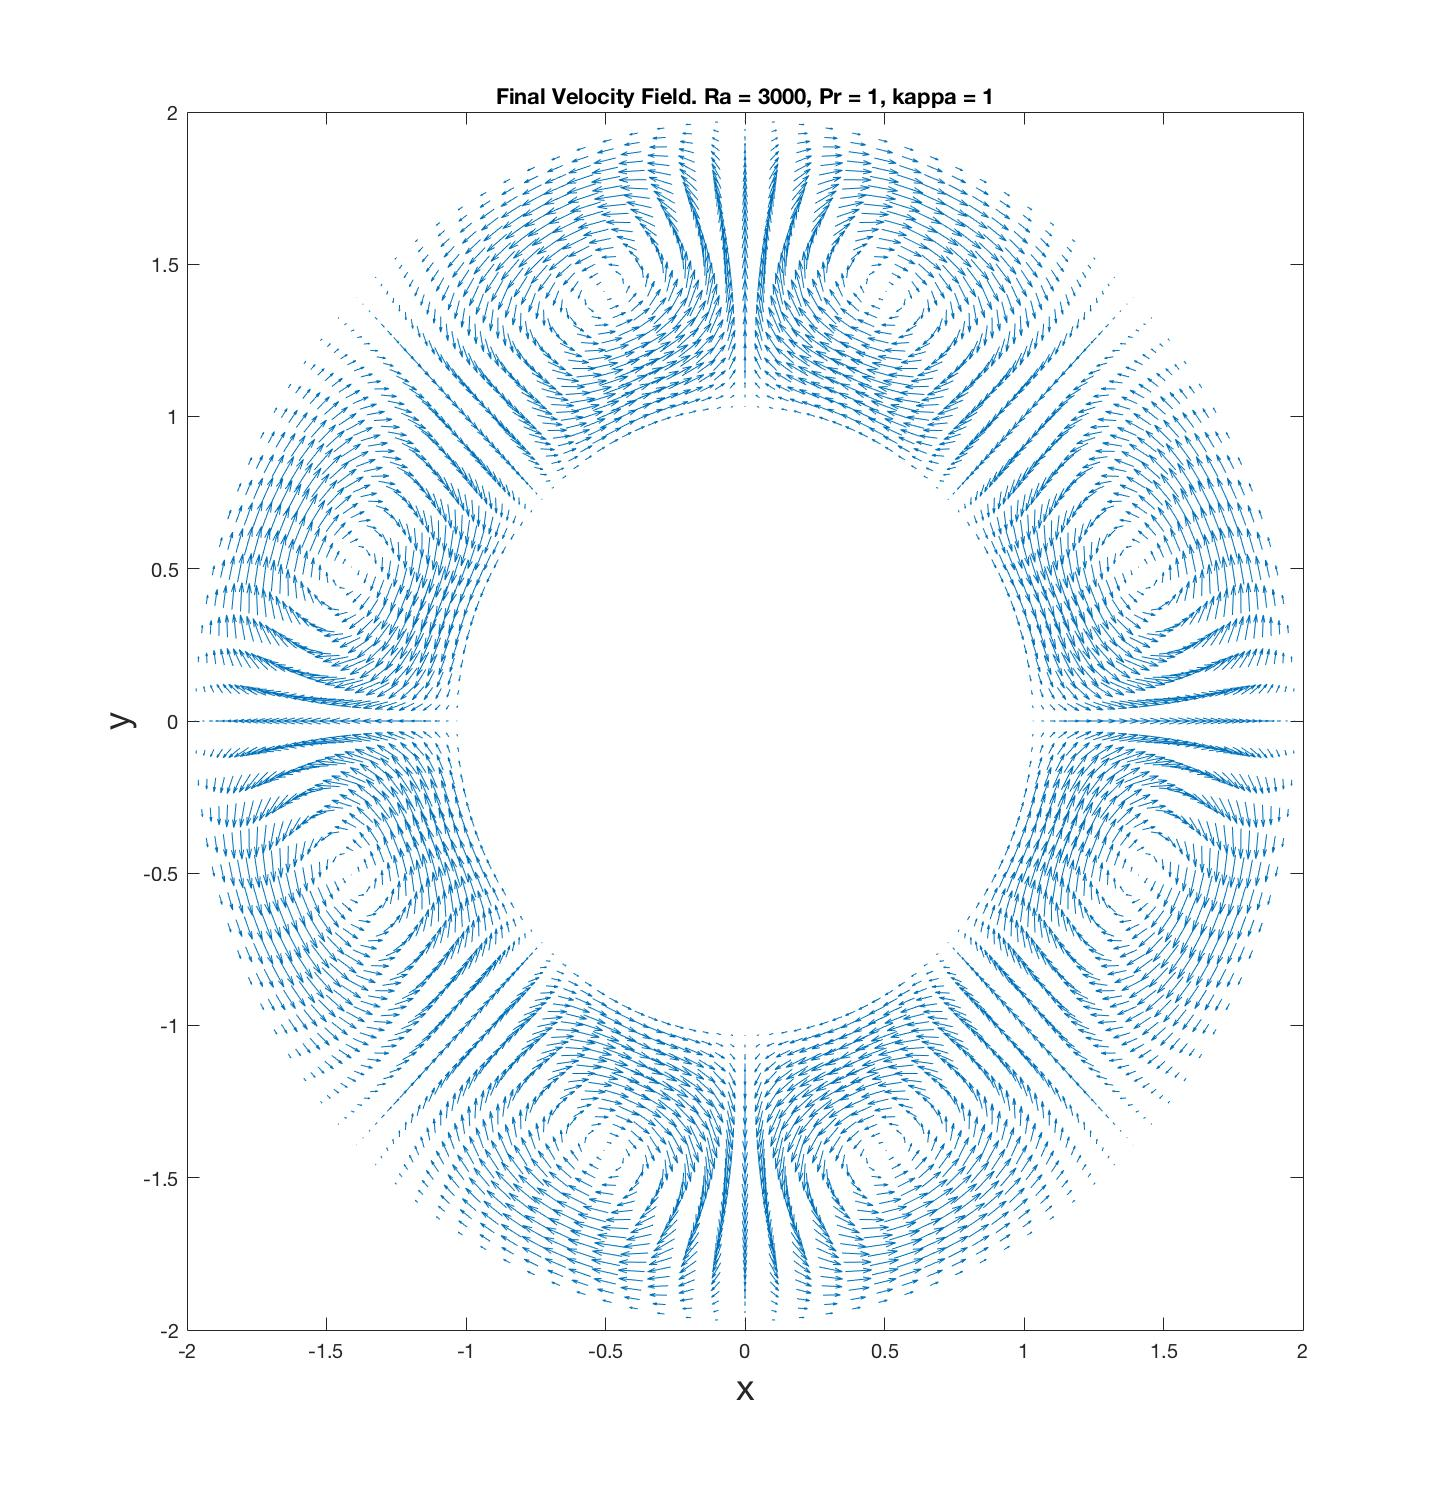
\includegraphics[width = 0.49\textwidth]{fig_q4ura3000}
		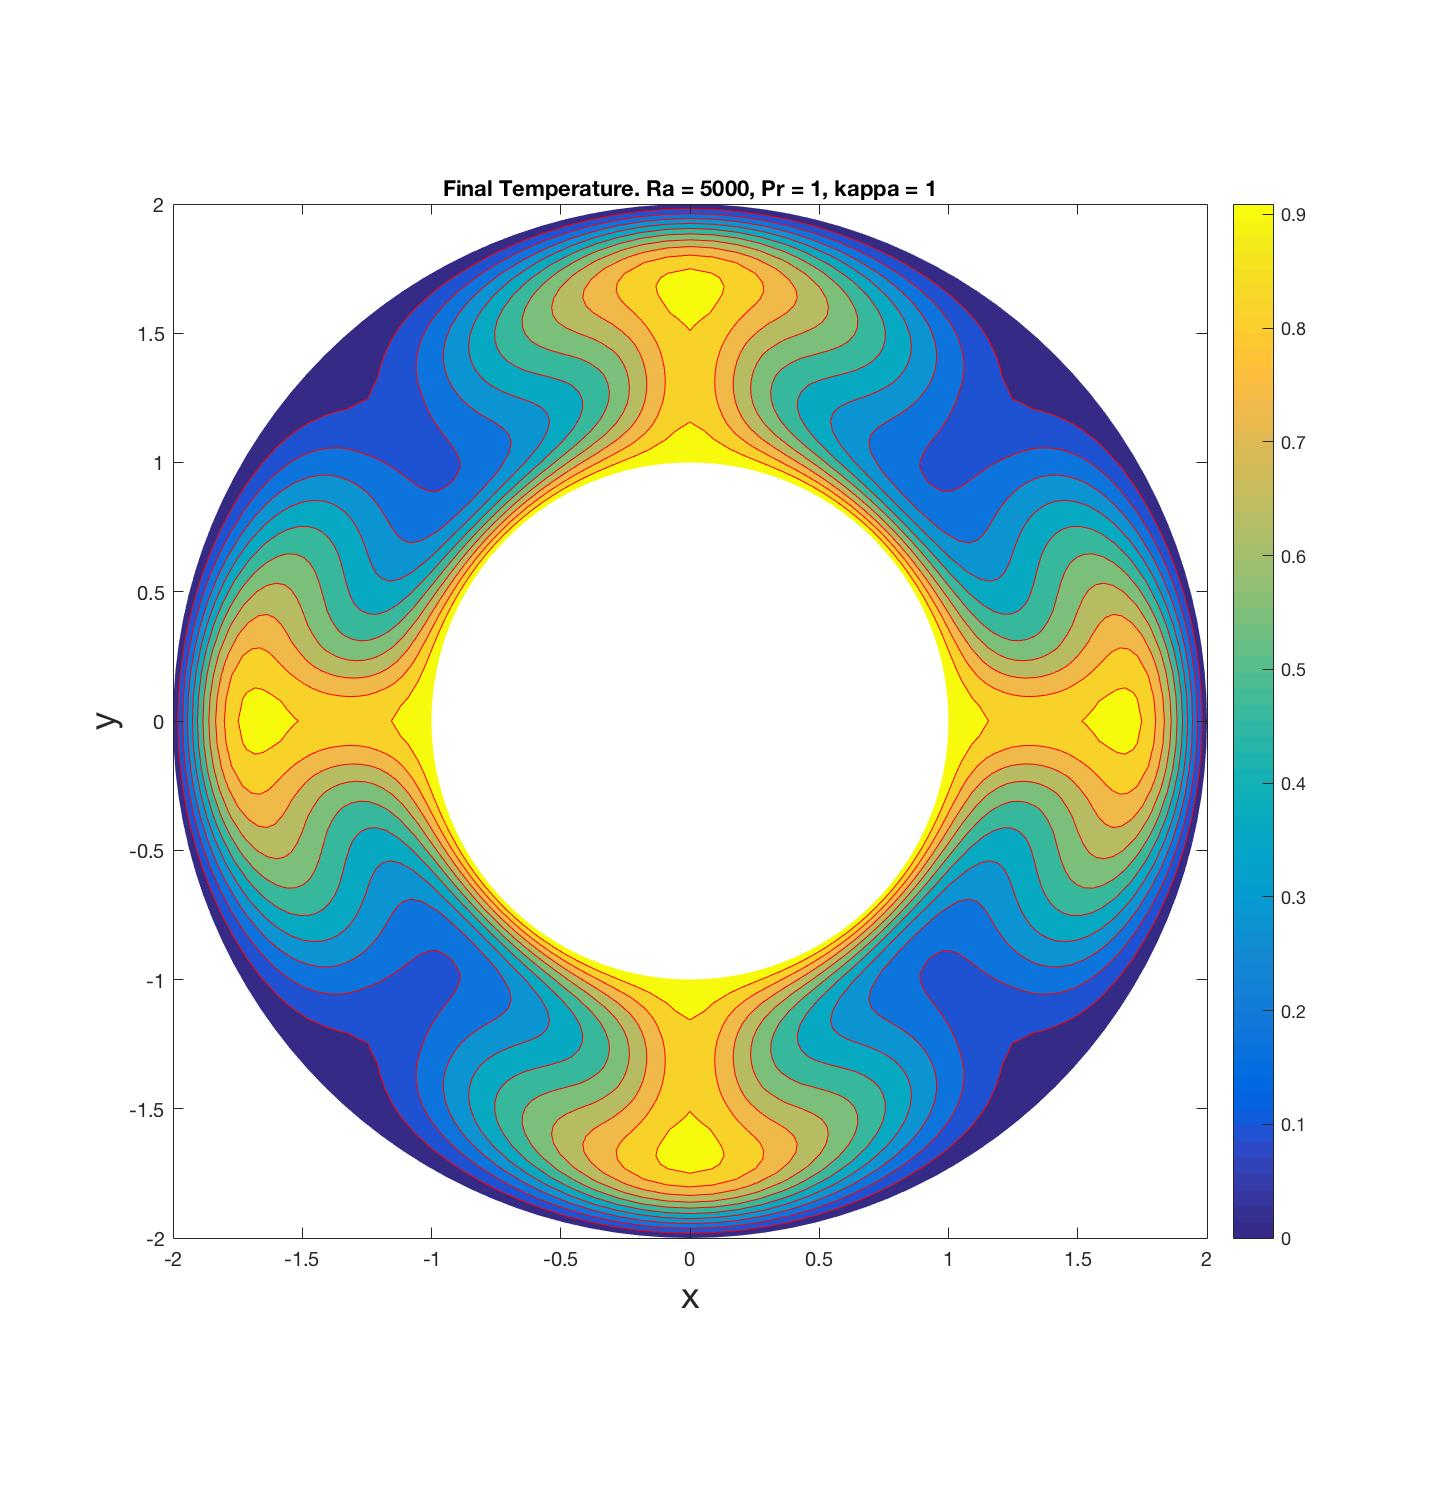
\includegraphics[width = 0.49\textwidth]{fig_q4ra5000}
		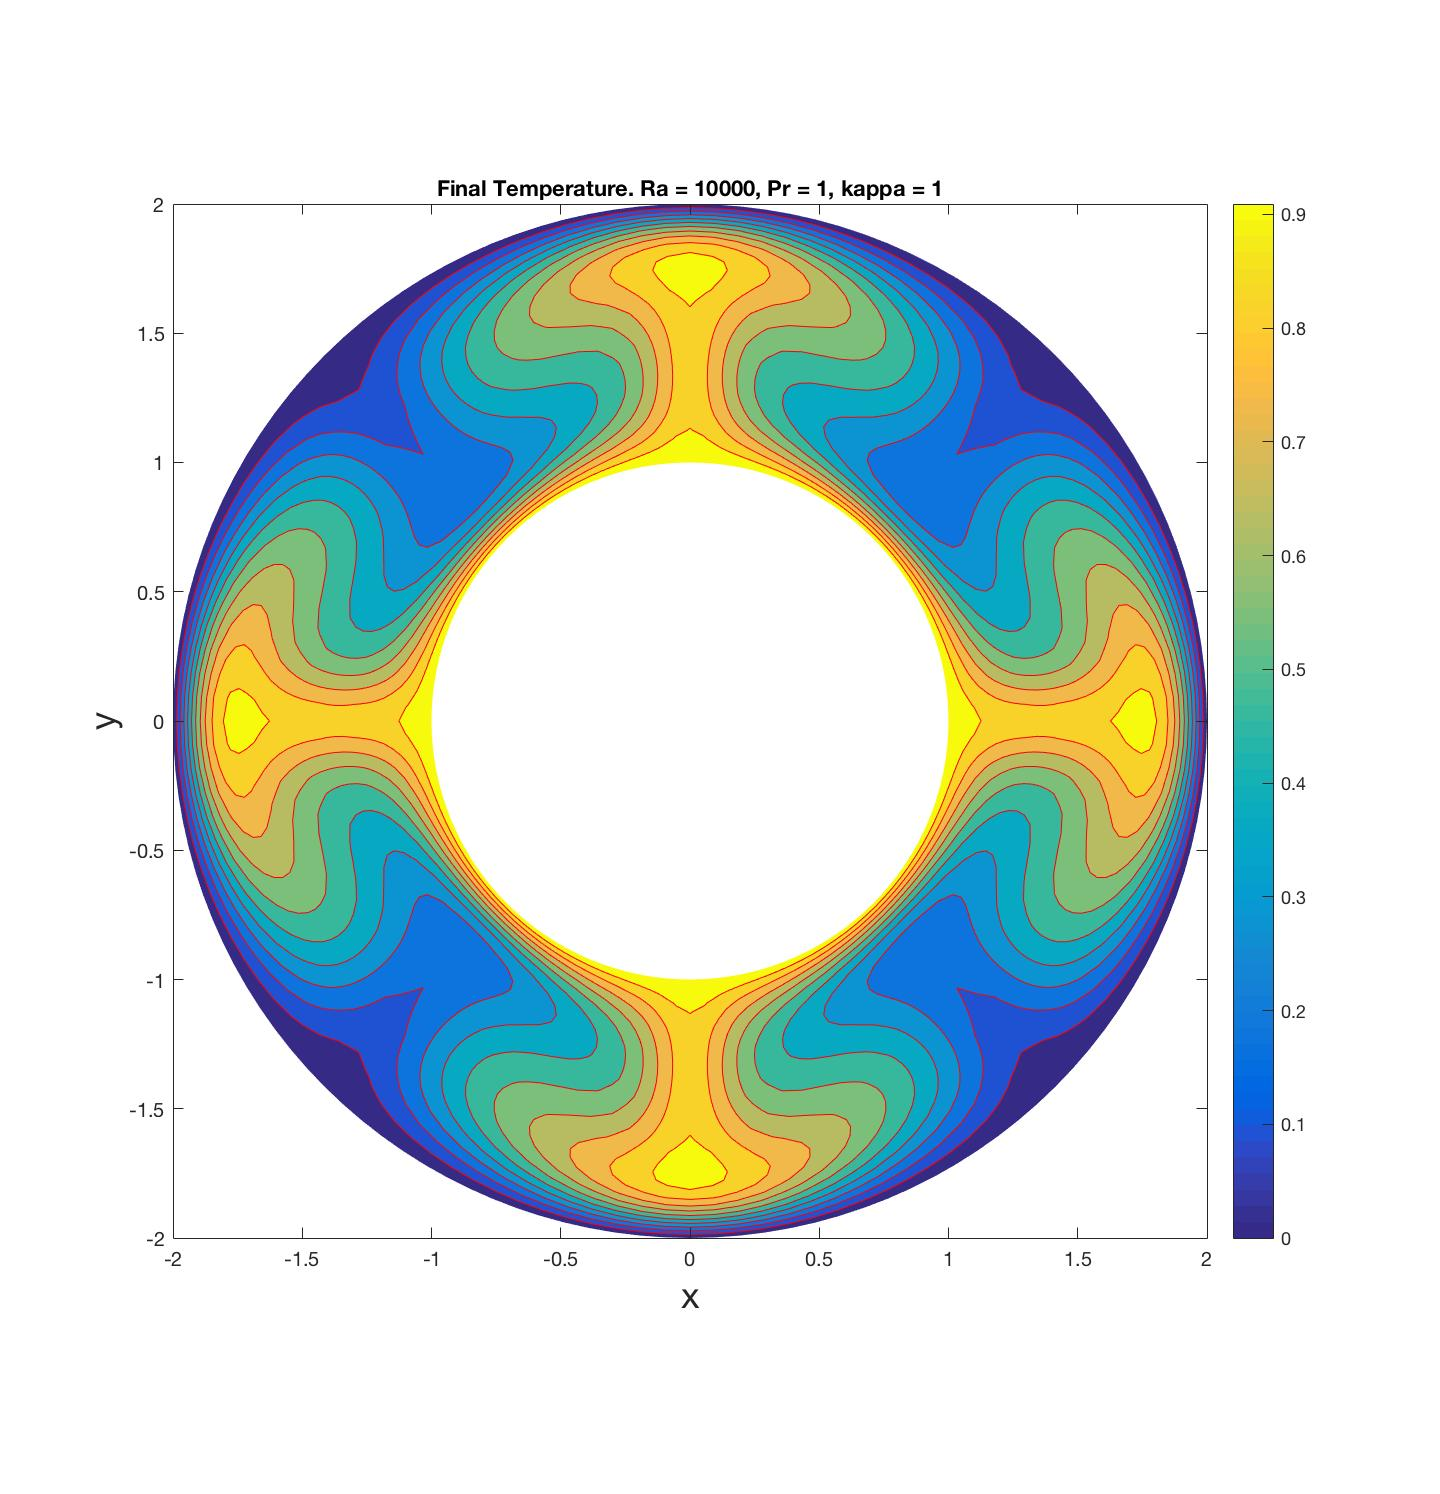
\includegraphics[width = 0.49\textwidth]{fig_q4ra10000}
		\caption{Q4: Final Temperature Field after solving the full problem for $P_r = \kappa = 1$ and $b=2$ for various values of $R_a$.}
		\label{fig:q4Rab2}
	\end{figure}
	%%%%%%%%%%%%%%%%%%%%%%%%%%%%%%%%%%%%%%%%%%%%%%%%%%%%%%%%%%%%

Now we consider the impact on the value of $R_c$ when changing the value of $b$. 

For $b=3$, and $b=5$ we get that $R_c \approx 300 $ (Figure \ref{fig:q4Rab3}) and $R_c \approx 25$ (Figure \ref{fig:q4Rab5}) respectively as well. So it seems that increasing the value of $b$ quickly decreases the value of $R_c$.  

	%%%%%%%%%%%%%%%%%%%%%%%%%%%%%%%%%%%%%%%%%%%%%%%%%%%%%%%%%%%%
	\begin{figure}[h!]
		\centering
		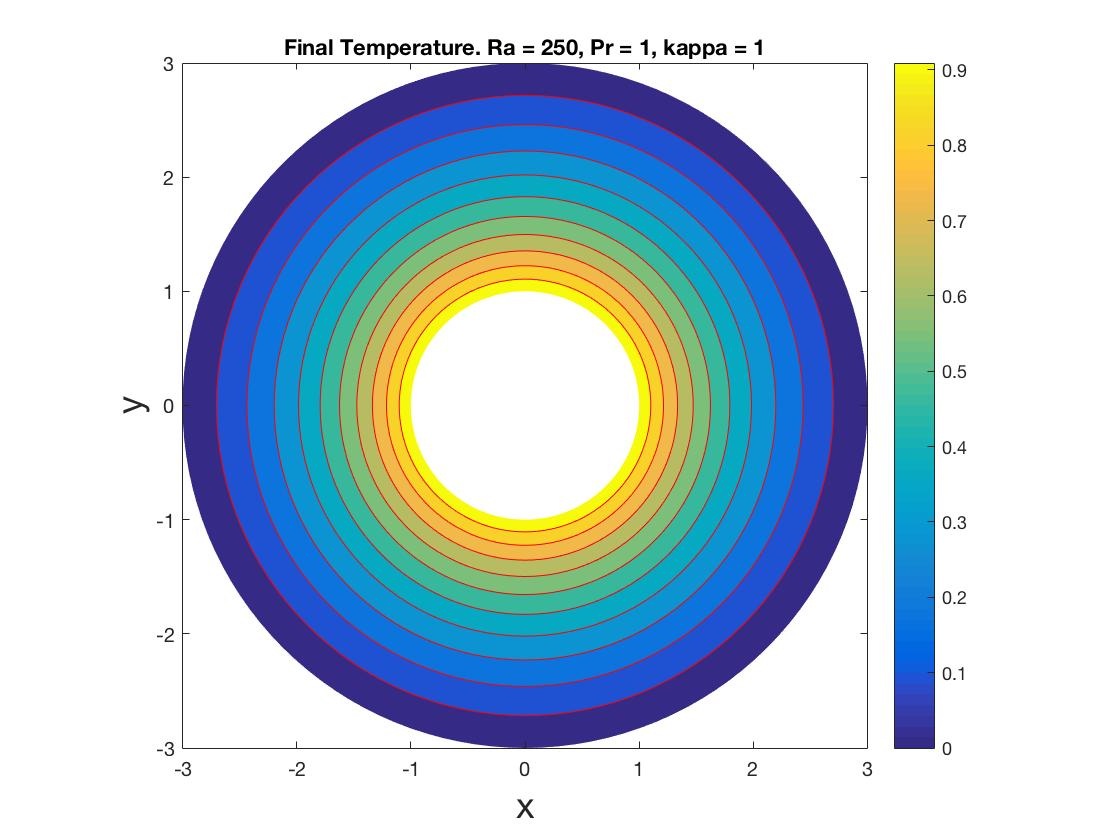
\includegraphics[width = 0.49\textwidth]{fig_q4ra250b3}
		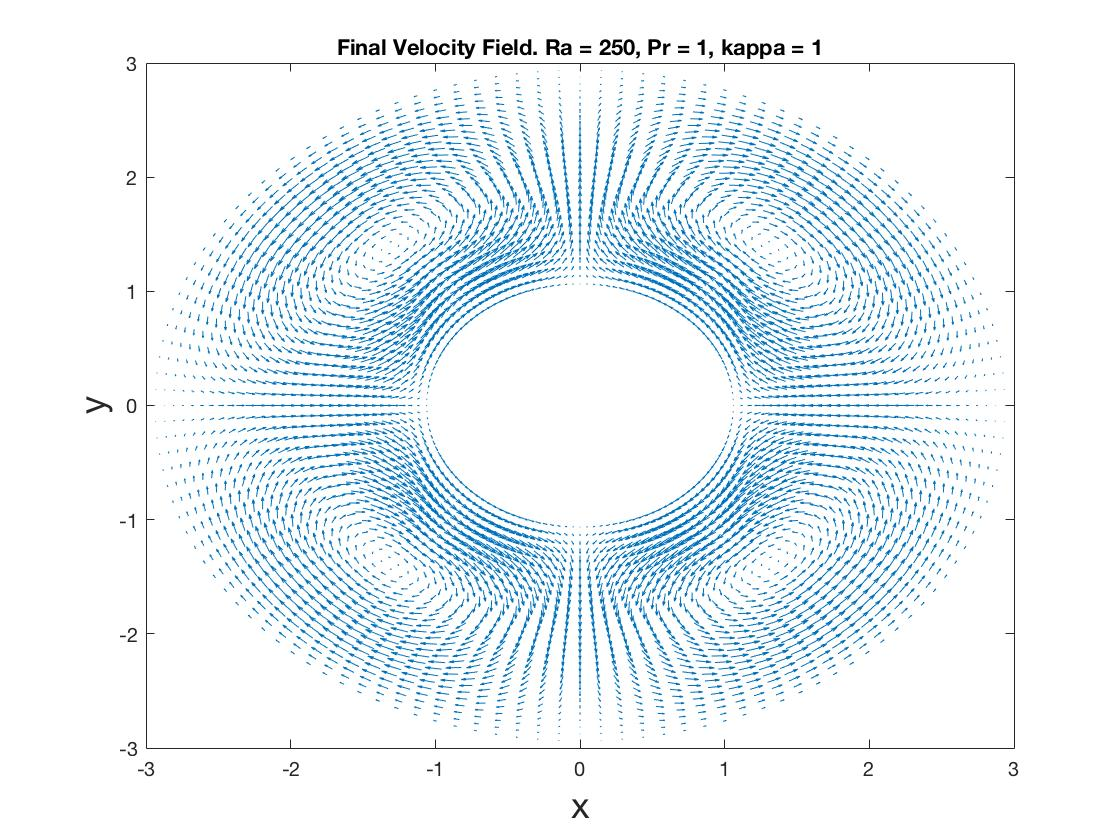
\includegraphics[width = 0.49\textwidth]{fig_q4ura250b3}
		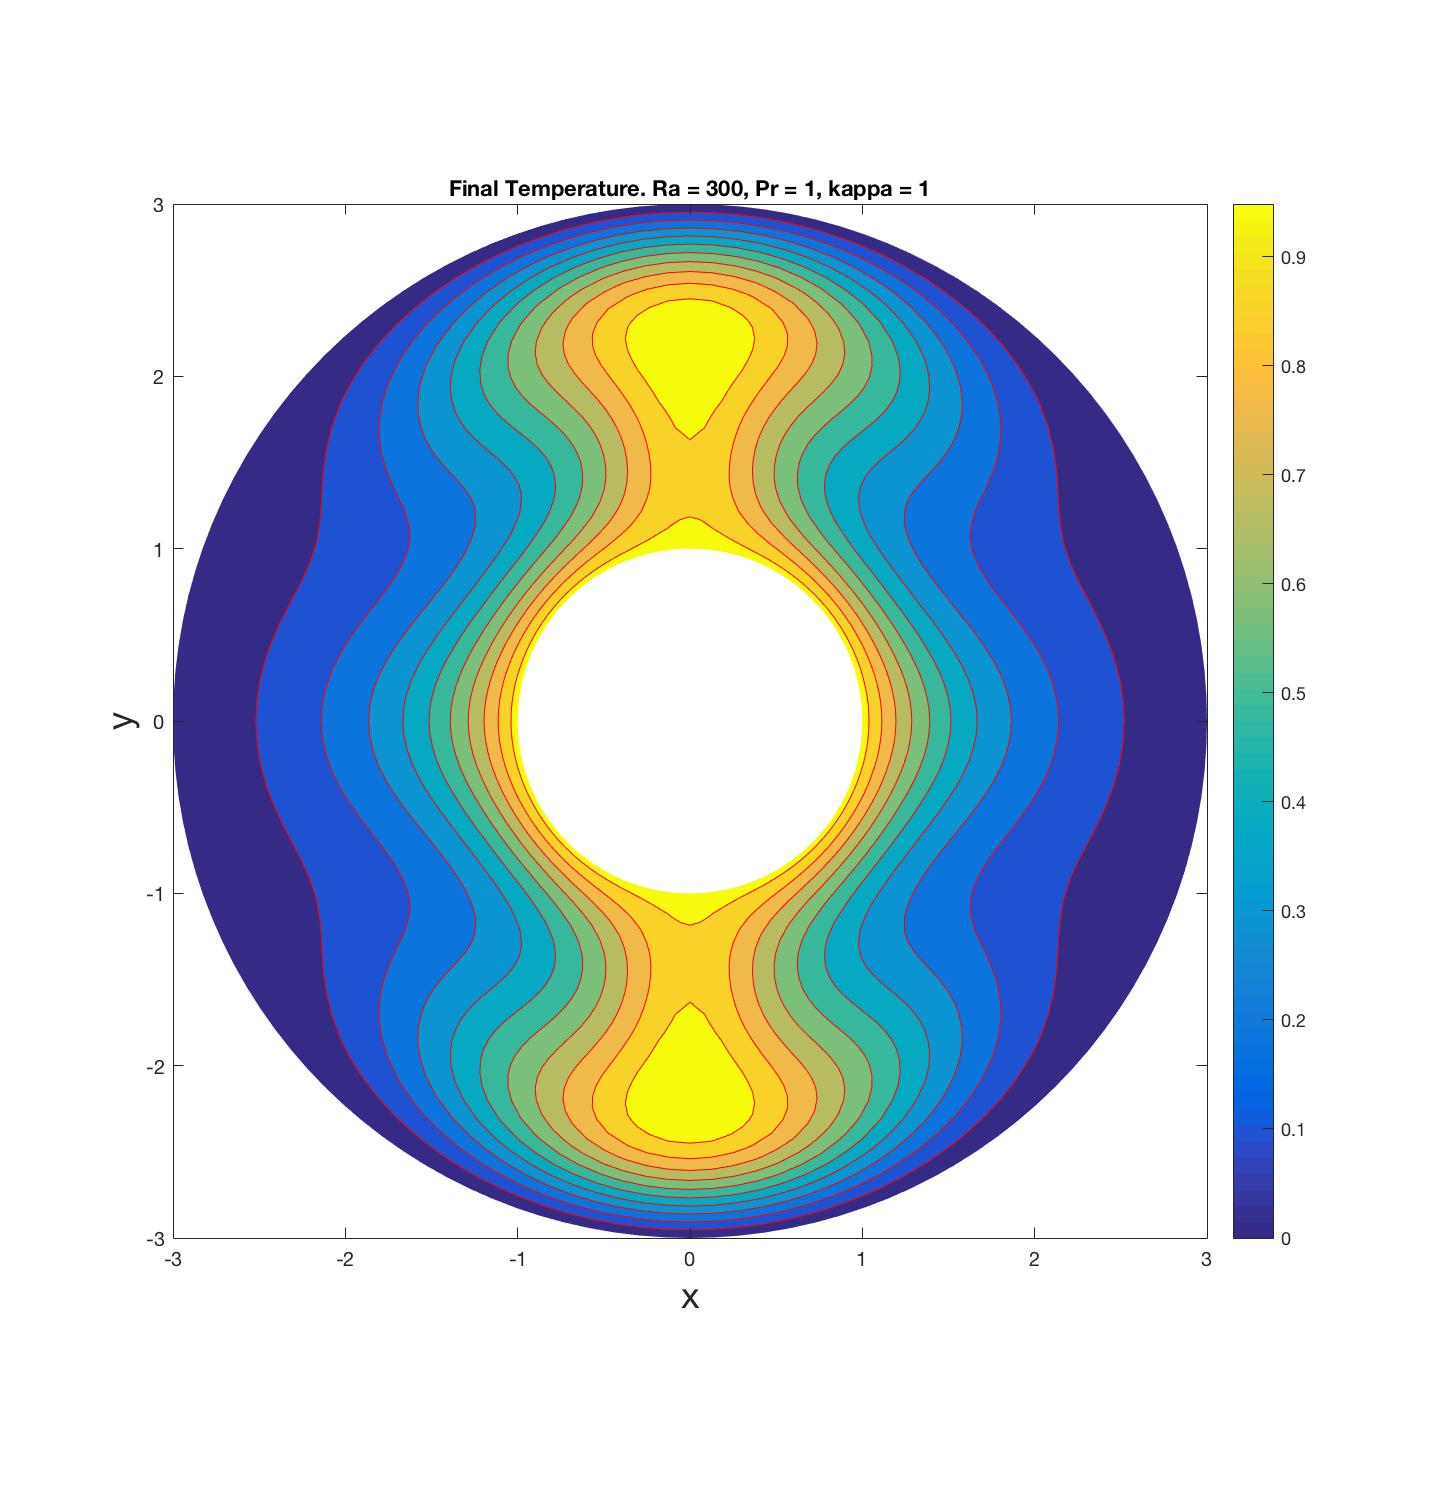
\includegraphics[width = 0.49\textwidth]{fig_q4ra300b3}
		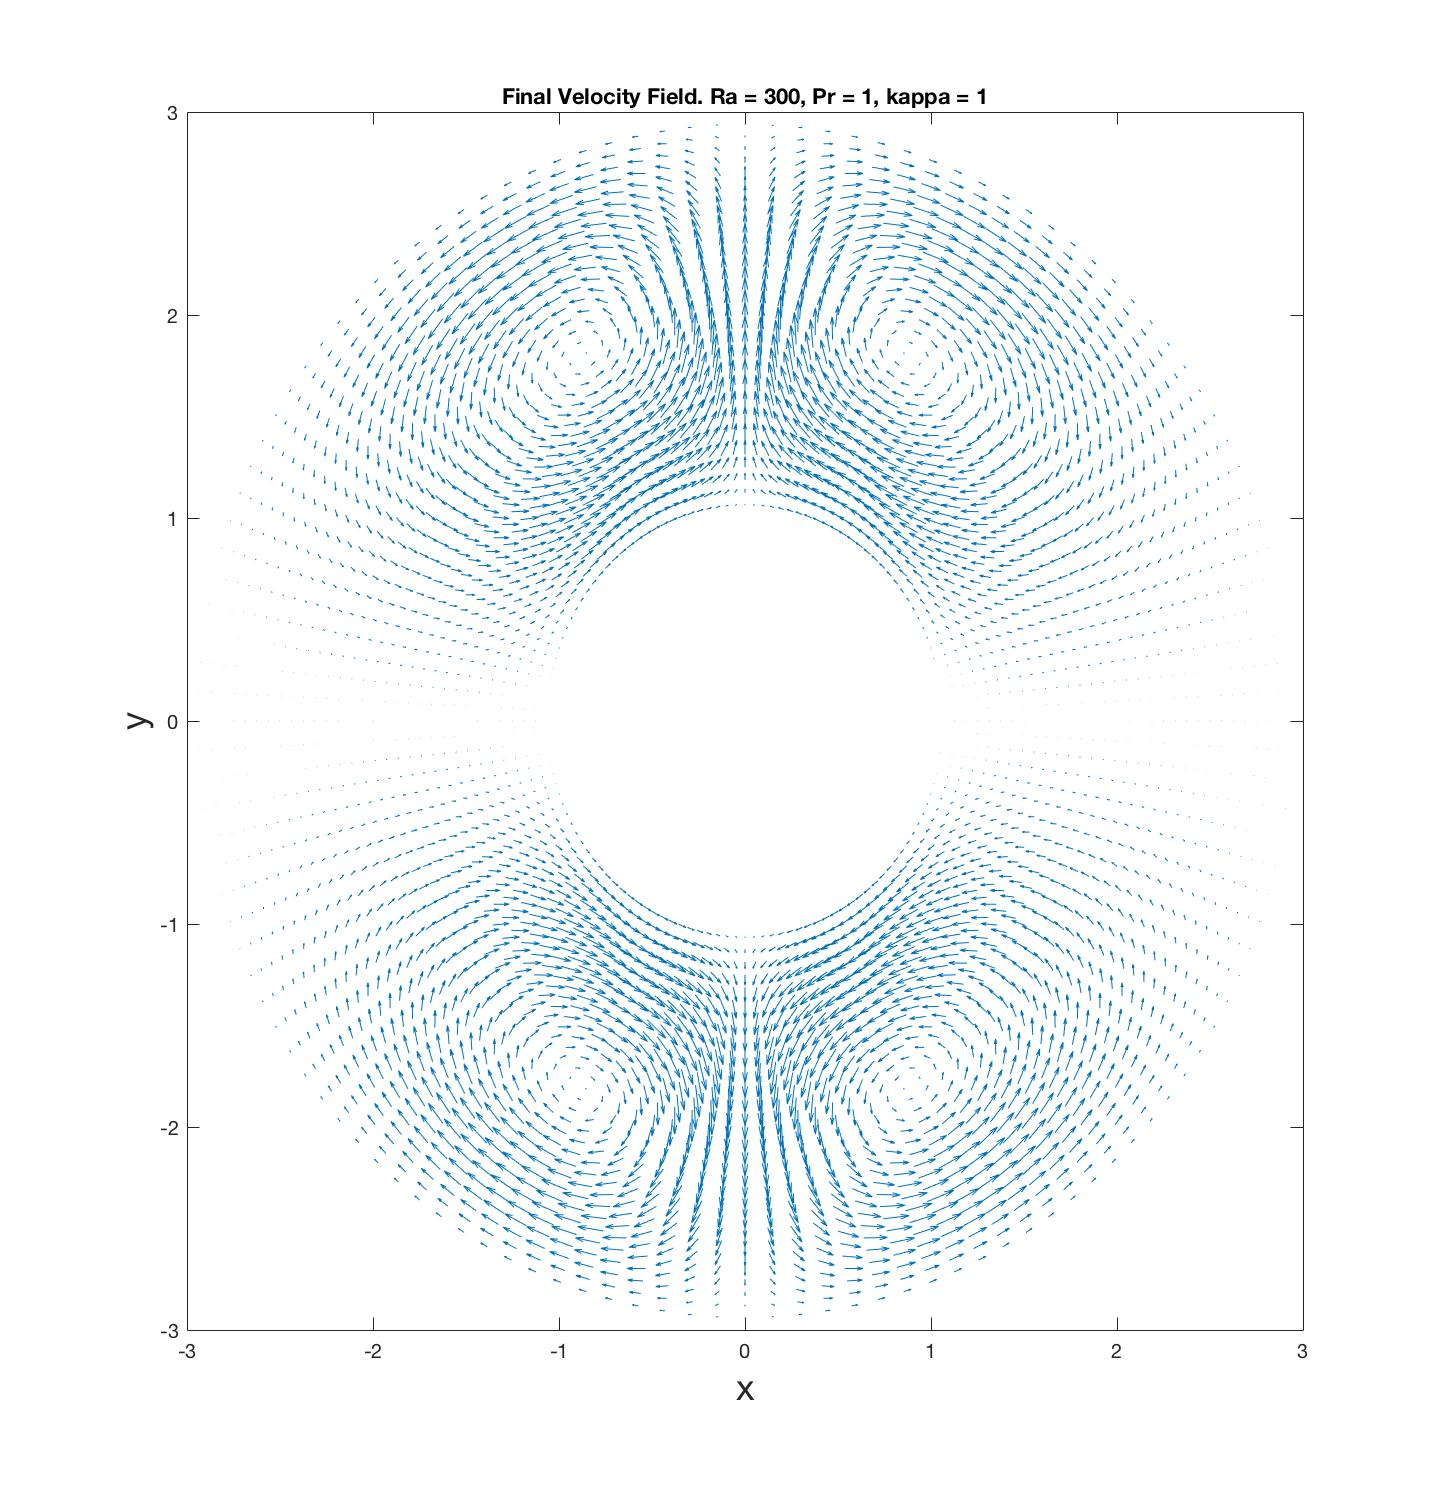
\includegraphics[width = 0.49\textwidth]{fig_q4ura300b3}
		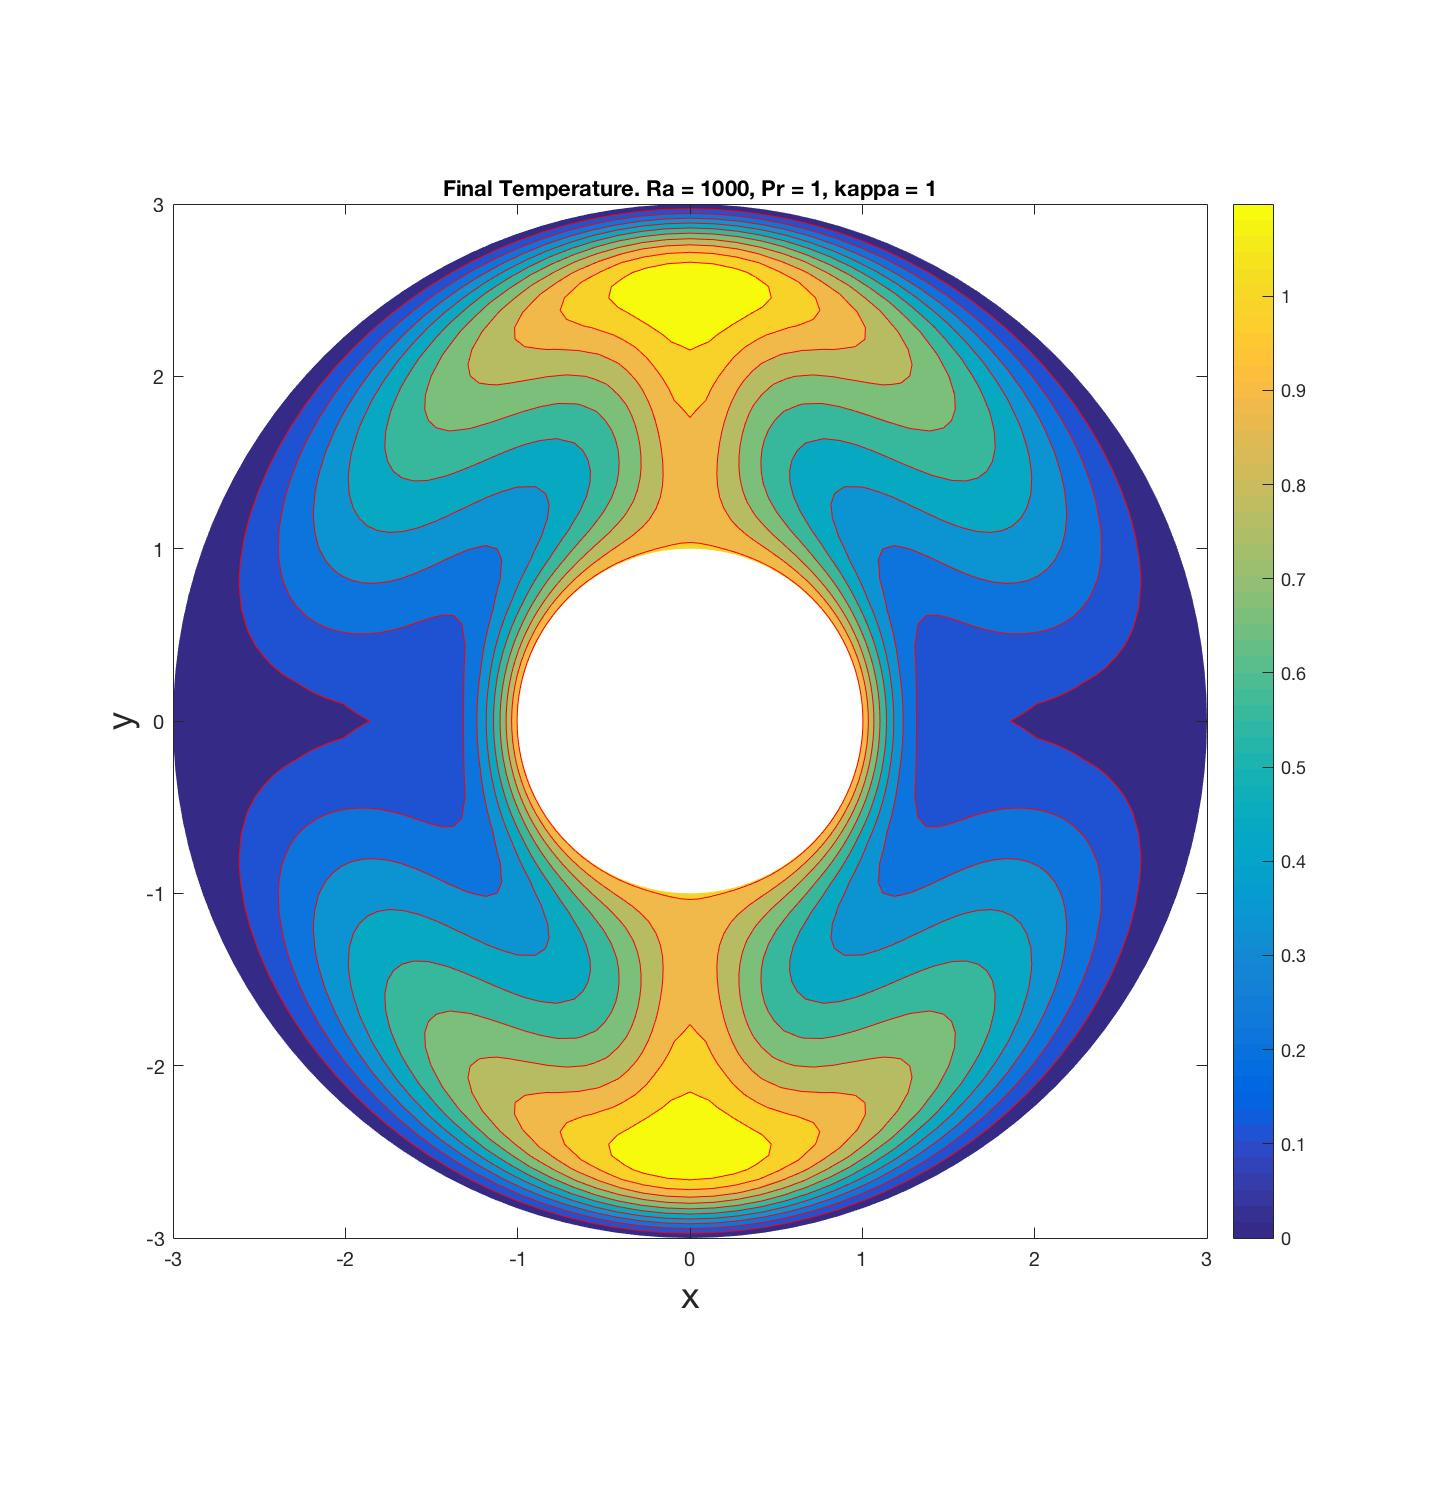
\includegraphics[width = 0.49\textwidth]{fig_q4ra1000b3}
		\caption{Q4: Final Temperature Field after solving the full problem for $P_r = \kappa = 1$ and $b=3$ for various values of $R_a$.}
		\label{fig:q4Rab3}
	\end{figure}
	%%%%%%%%%%%%%%%%%%%%%%%%%%%%%%%%%%%%%%%%%%%%%%%%%%%%%%%%%%%%

	%%%%%%%%%%%%%%%%%%%%%%%%%%%%%%%%%%%%%%%%%%%%%%%%%%%%%%%%%%%%
	\begin{figure}[h!]
		\centering
		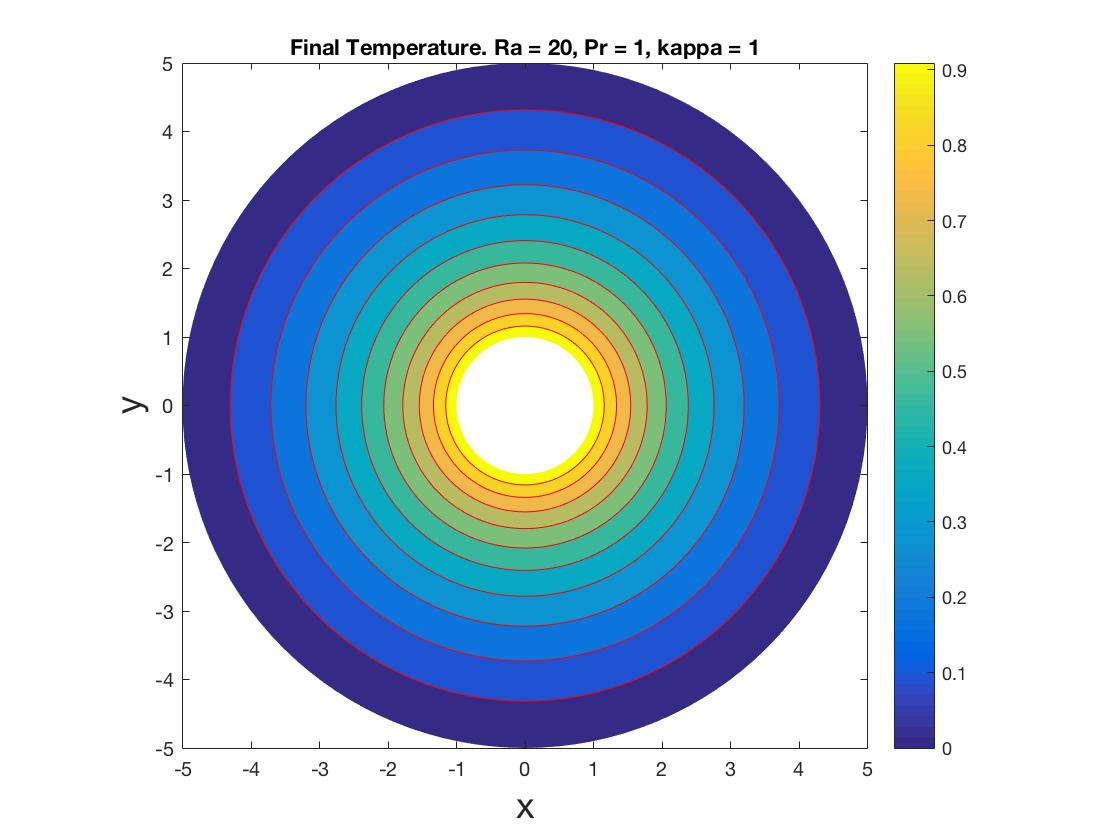
\includegraphics[width = 0.49\textwidth]{fig_q4ra20b5}
		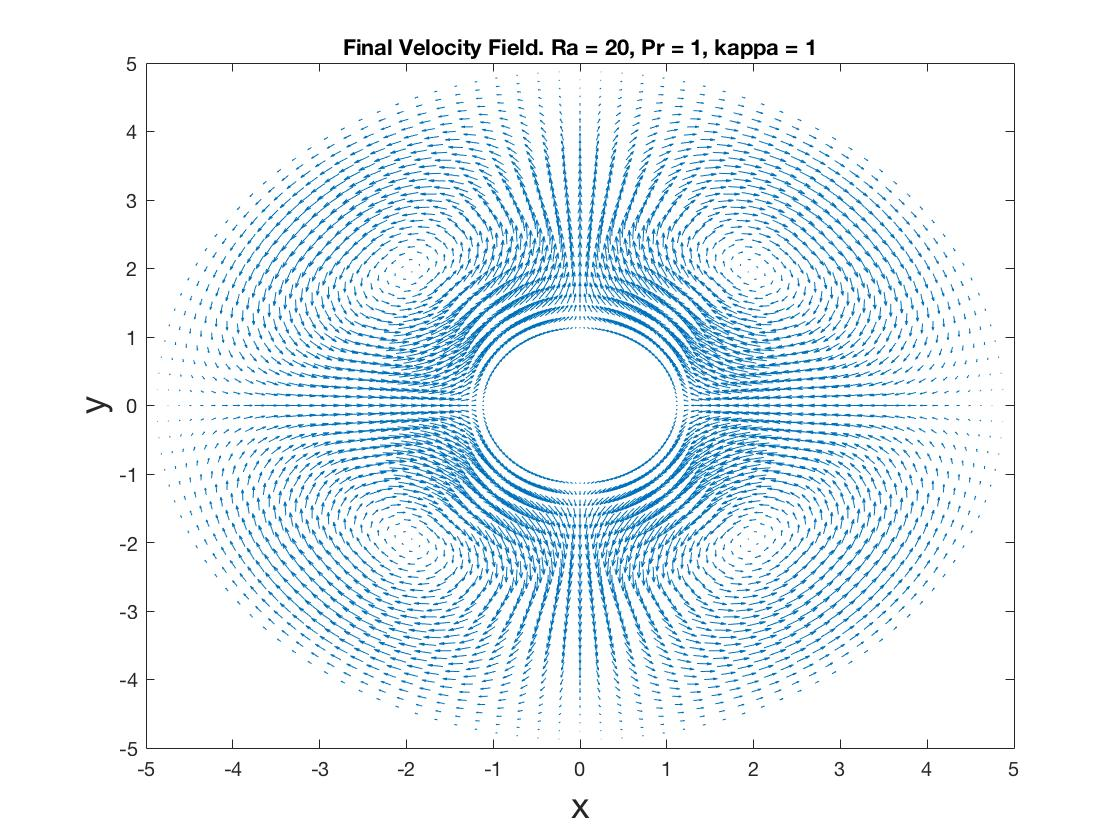
\includegraphics[width = 0.49\textwidth]{fig_q4ura20b5}
		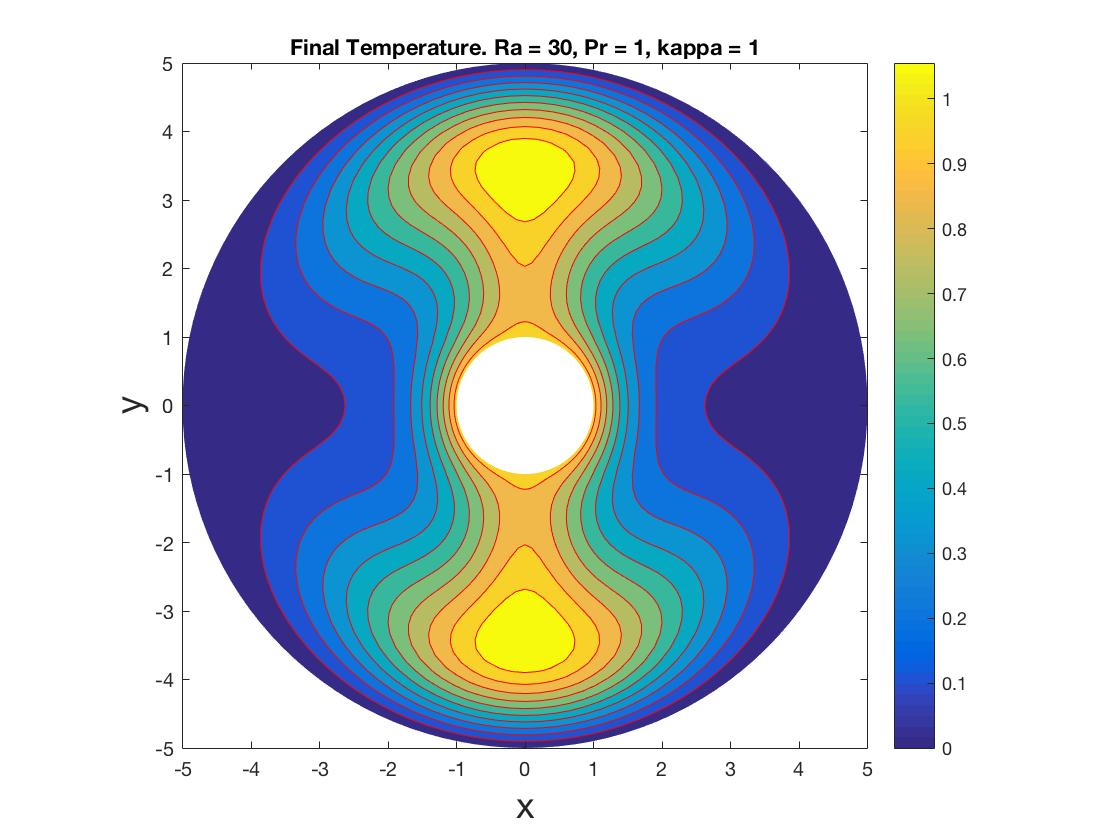
\includegraphics[width = 0.49\textwidth]{fig_q4ra30b5}
		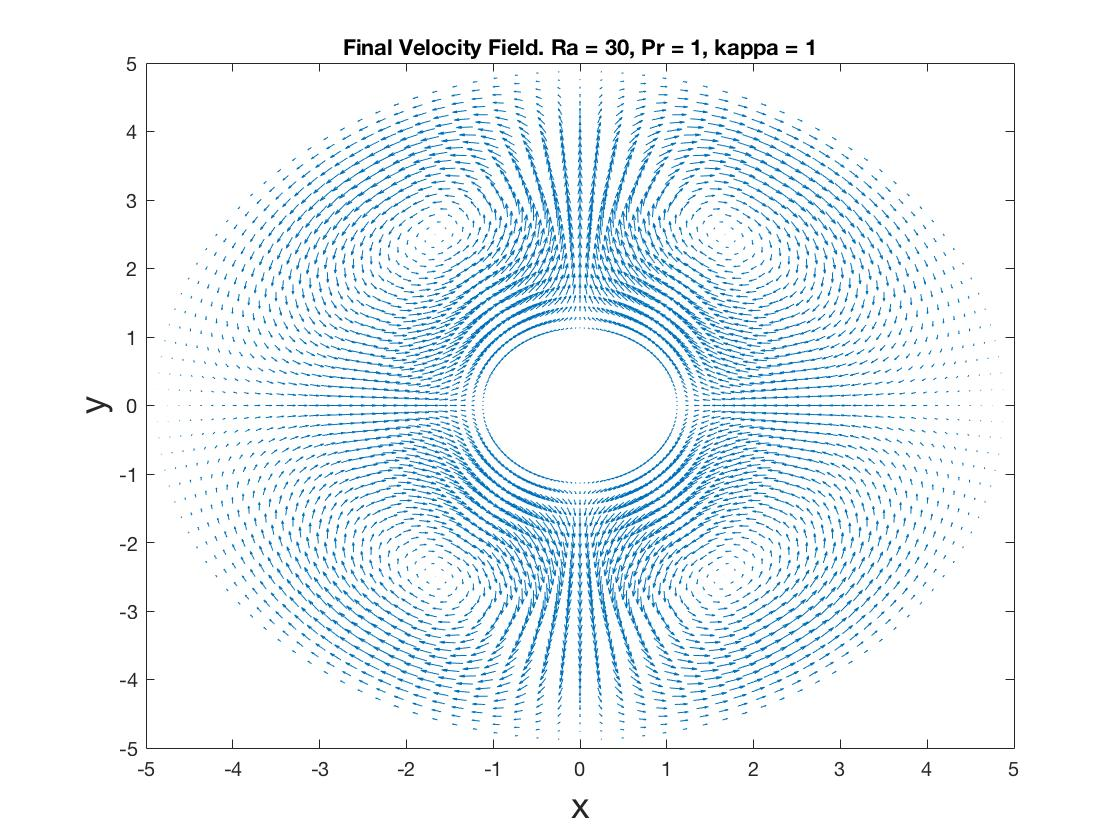
\includegraphics[width = 0.49\textwidth]{fig_q4ura30b5}
		\caption{Q4: Final Temperature Field after solving the full problem for $P_r = \kappa = 1$ and $b=5$ for various values of $R_a$.}
		\label{fig:q4Rab5}
	\end{figure}
	%%%%%%%%%%%%%%%%%%%%%%%%%%%%%%%%%%%%%%%%%%%%%%%%%%%%%%%%%%%%


\subsection{Varying $P_r$}

Choosing a small value of $P_r$ reduces the impact of thermal diffusivity which in turn results in a smaller impact from the thermal driving force. So going back to $b=2$, it can be seen in Figure \ref{fig:q4pr001} that even for $R_a = 10000$ when $P_r = 0.01$, the solution converges to no rolls.  Even for $b=3$, with $R_a = 500$ and with $P_r = 0.01$, no rolls appear. 

	%%%%%%%%%%%%%%%%%%%%%%%%%%%%%%%%%%%%%%%%%%%%%%%%%%%%%%%%%%%%
	\begin{figure}[h!]
		\centering
		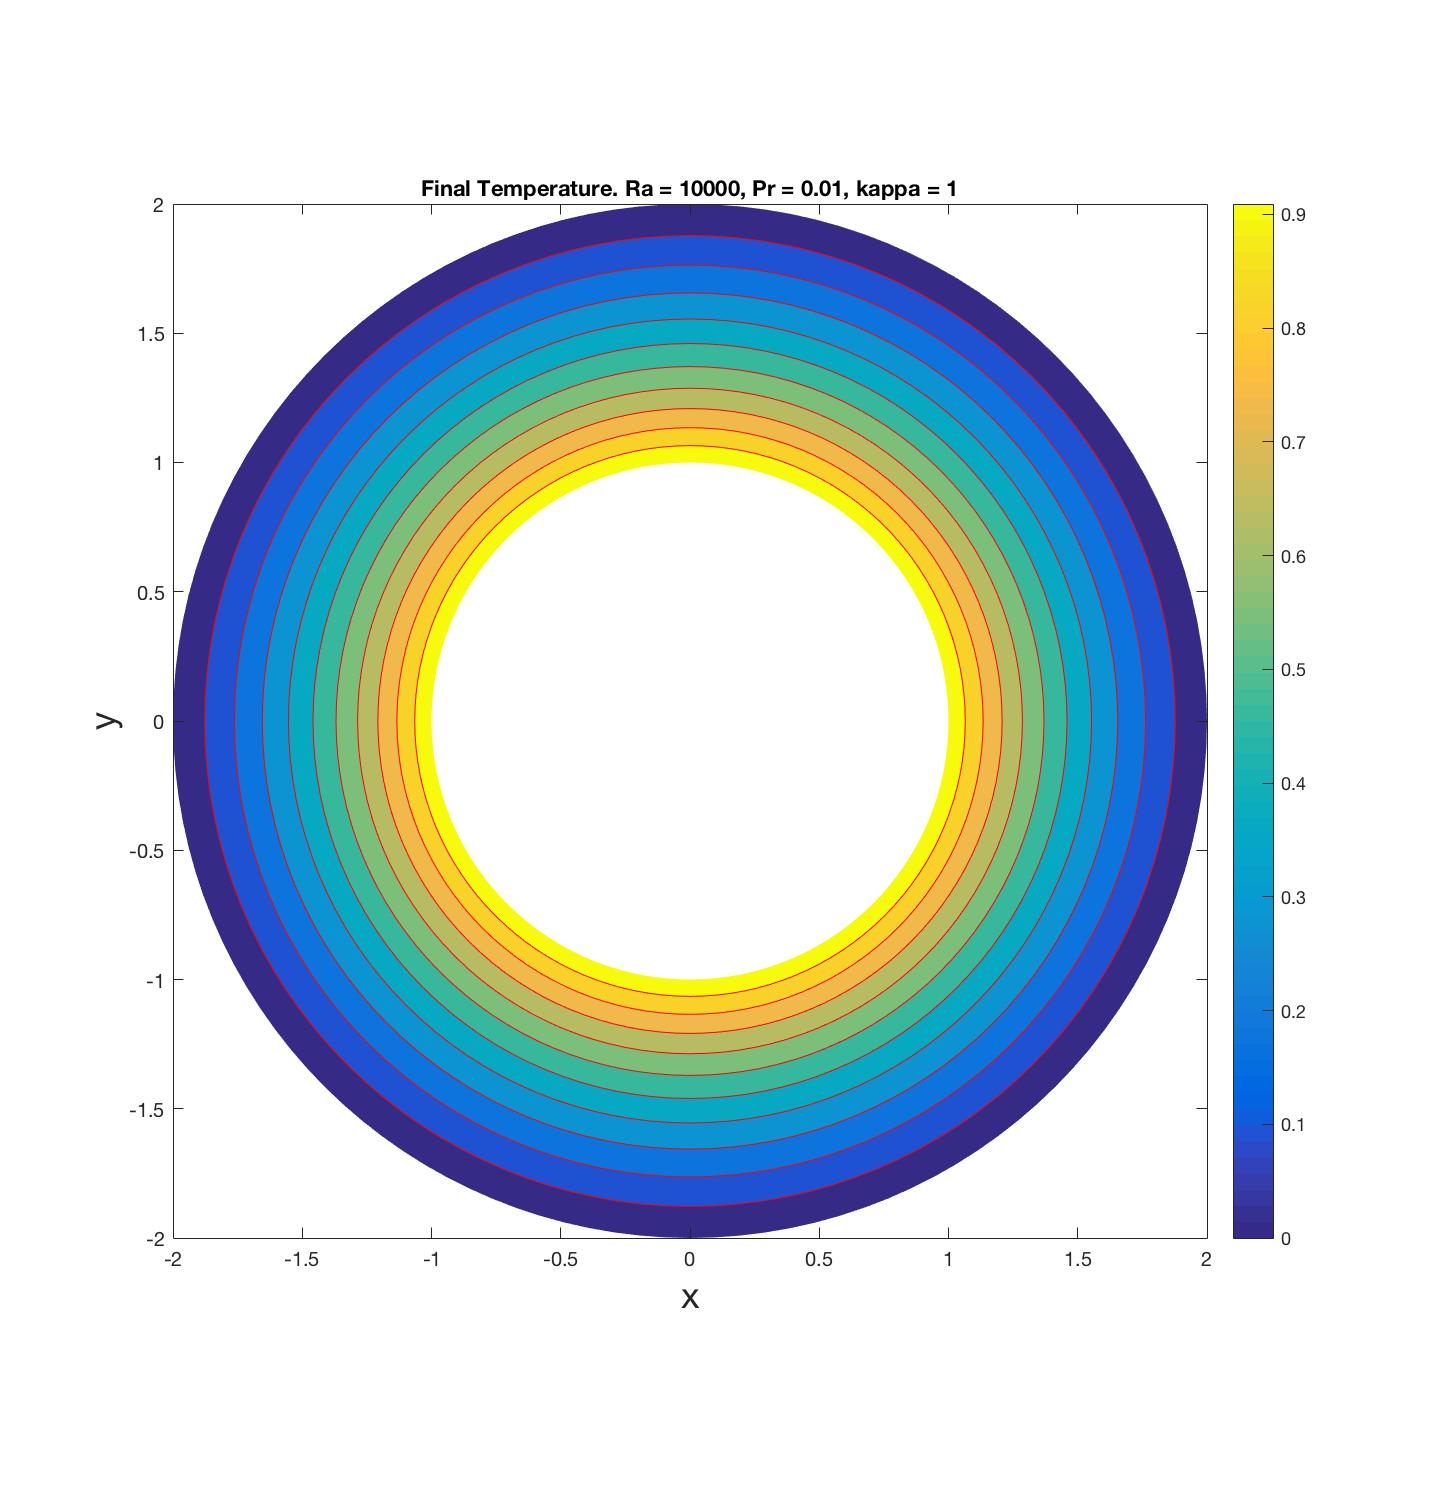
\includegraphics[width = 0.49\textwidth]{fig_q4pr001}
		\caption{Q4: Final Temperature Field after solving the full problem for $P_r = 0.01, R_a = 10000$ and $b=2$.}
		\label{fig:q4pr001}
	\end{figure}
	%%%%%%%%%%%%%%%%%%%%%%%%%%%%%%%%%%%%%%%%%%%%%%%%%%%%%%%%%%%%
	
	%%%%%%%%%%%%%%%%%%%%%%%%%%%%%%%%%%%%%%%%%%%%%%%%%%%%%%%%%%%%
	\begin{figure}[h!]
		\centering
		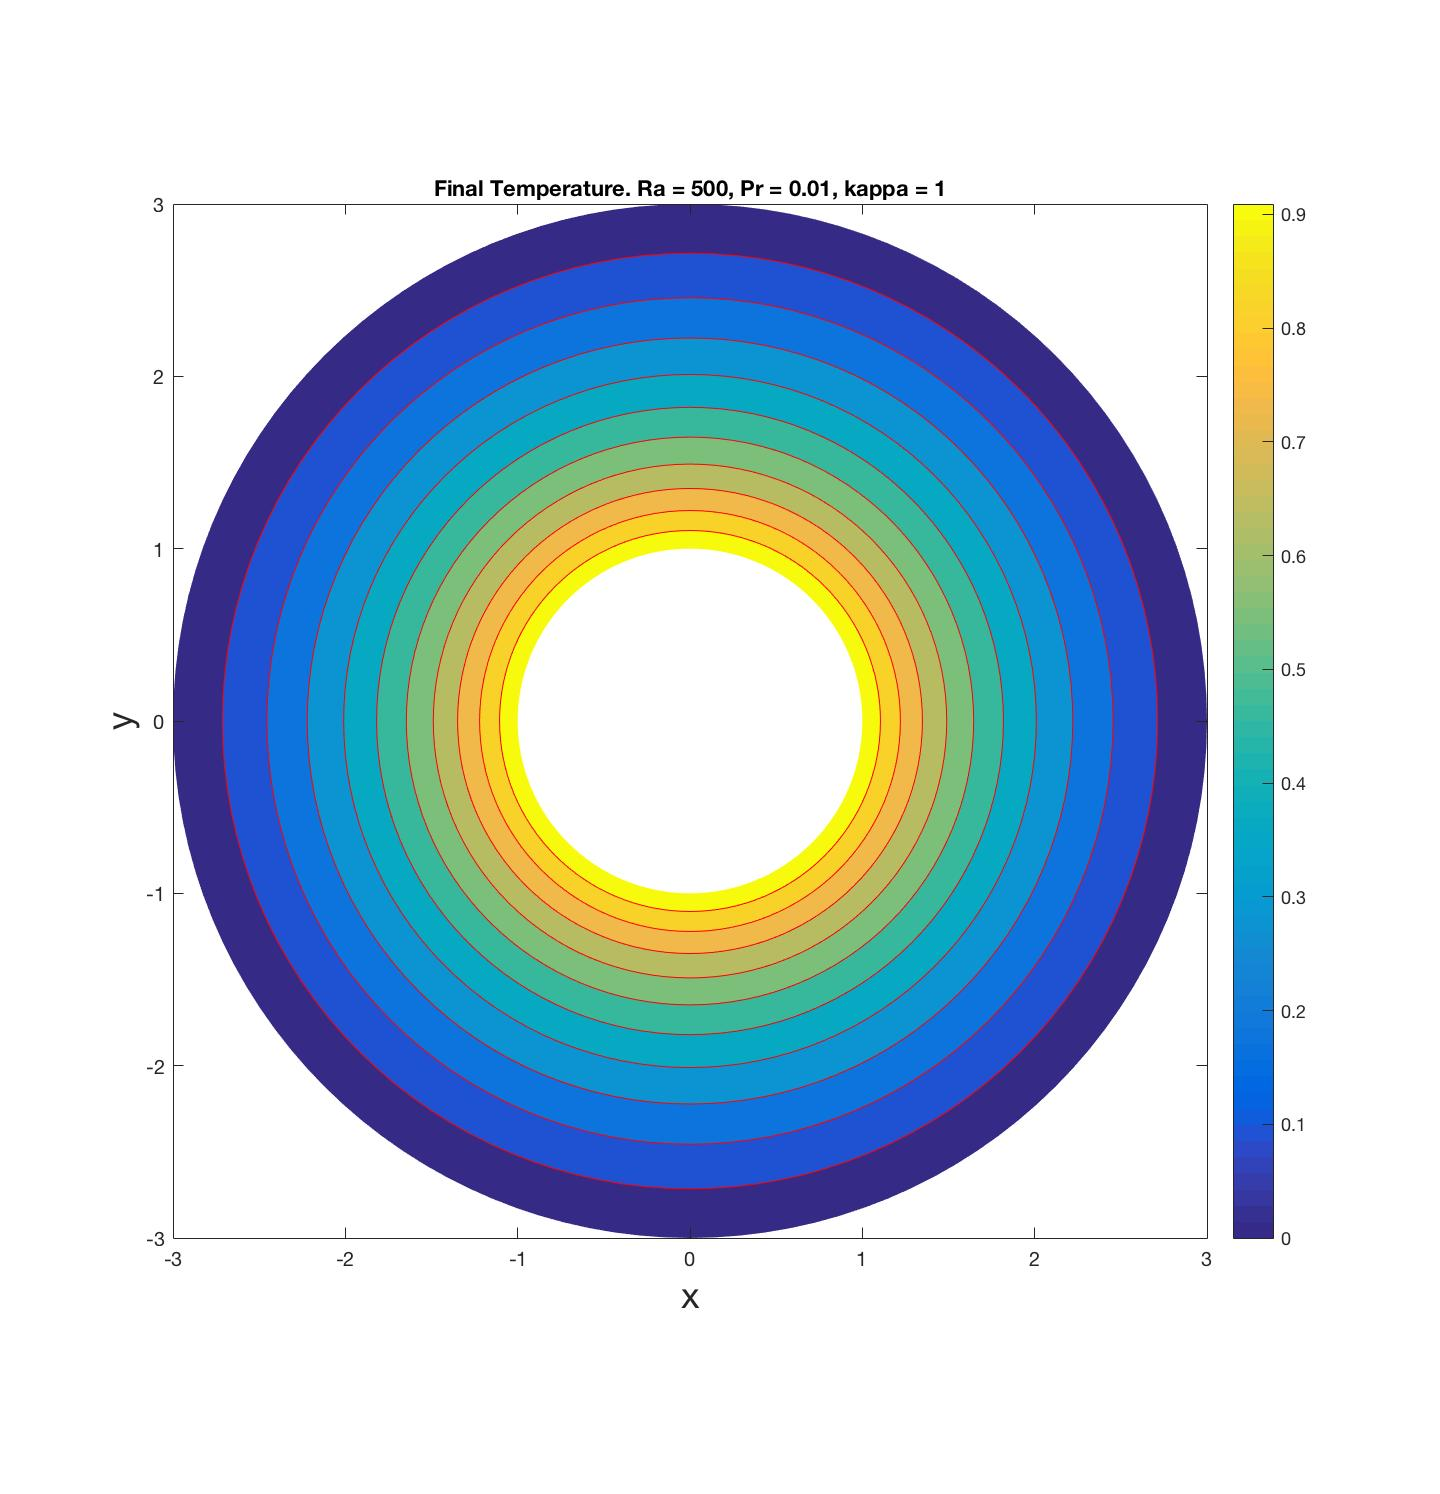
\includegraphics[width = 0.49\textwidth]{fig_q4pr001b3}
		\caption{Q4: Final Temperature Field after solving the full problem for $P_r = 0.01, R_a = 500$ and $b=3$.}
		\label{fig:q4pr001}
	\end{figure}
	%%%%%%%%%%%%%%%%%%%%%%%%%%%%%%%%%%%%%%%%%%%%%%%%%%%%%%%%%%%%
	
Based on these results I believe the ratio between $P_r$ and $R_a$ matters as well as than the individual values themselves.

\subsection{Conclusion}

The number of rolls are impacted by the chosen values of $R_a, P_r,$ and $b$.

Finally it is worth noting that a lot of the derived results are specific to the initial conditions and vary massively from situation to the situation. But nevertheless, it seems that the entire routine is function sufficiently and thus can be used, given enough time, to solve any specified problem of this type. 

\end{document}
